\chapter{Long-baseline Neutrino Oscillation Physics}
\label{ch:physics-lbnosc}

\section{Context}
\label{sec:physics-lbnosc-context}

% {\bf [Note: Copied from Section 2.2 of the LBNE Science Document.]}  
The Standard Model of particle physics 
presents a remarkably accurate
description of the elementary particles and their
interactions. However, its limitations beg deeper questions about
Nature. The unexplained patterns of quarks, leptons, flavors and
generations imply that a more fundamental underlying theory must
exist.  
DUNE plans to pursue a detailed
study of neutrino mixing, resolve the neutrino mass ordering,
and search for CP violation in the lepton sector by
studying the oscillation patterns of high-intensity
$\nu_\mu$ and $\overline{\nu}_\mu$ beams measured over a long baseline. 
Neutrino oscillation arises from mixing between the flavor and mass eigenstates of neutrinos,
corresponding to the weak and gravitational interactions, respectively. 
This three-flavor-mixing
scenario can be described by a rotation between the weak-interaction
eigenstate basis $(\nu_e,\, \nu_\mu,\, \nu_\tau)$ and the basis of
states of definite mass $(\nu_1,\, \nu_2,\, \nu_3)$.  In direct
correspondence with mixing in the quark sector, the transformations
between basis states is expressed in the form of a complex unitary
matrix, known as the PMNS matrix :
\begin{equation}
\left(\begin{array}{ccc} \nu_e \\ \nu_\mu \\ \nu_\tau \end{array} \right)= 
\underbrace{
  \left(\begin{array}{ccc}
      U_{e 1} &  U_{e 2} & U_{e 3} \\ 
      U_{\mu1} &  U_{\mu2} & U_{\mu 3} \\ 
      U_{\tau 1} &  U_{\tau 2} & U_{\tau 3} 
    \end{array} \right)
}_{U_{\rm PMNS}} \left(\begin{array}{ccc} \nu_1 \\ \nu_2 \\ \nu_3 \end{array} \right).
\label{eqn:pmns0}
\end{equation}
The PMNS matrix in full generality depends on just three mixing angles
and a CP-violating phase.  The mixing angles and phase are designated
as $(\theta_{12},\, \theta_{23},\, \theta_{13})$ and
\deltacp.  %\fixme{mathmatical rep of mixing}
This matrix can be parameterized as the product of three
two-flavor mixing matrices as follows, where $c_{\alpha \beta}=\cos \theta_{\alpha \beta}$ and $s_{\alpha
  \beta}=\sin \theta_{\alpha \beta}$:

\begin{equation}
U_{\rm PMNS} = 
  \underbrace{
    \left( \begin{array}{ccc}
        1 & 0 & 0 \\ 
        0 & c_{23} & s_{23} \\ 
        0 & -s_{23} & c_{23}
    \end{array} \right)
  }_{\rm I}
\underbrace{
  \left( \begin{array}{ccc}
      c_{13} & 0 & e^{i\delta_{cp}}s_{13} \\ 
      0 & 1 & 0 \\ 
      -e^{i\delta_{cp}}s_{13} & 0 & c_{13}
  \end{array} \right) 
}_{\rm II}
\underbrace{
 \left( \begin{array}{ccc}
      c_{12} & s_{12} & 0 \\ 
      -s_{12} & c_{12} & 0 \\ 
      0 & 0 & 1
  \end{array} \right) 
}_{\rm III}
\label{eqn:pmns}
\end{equation}
The parameters of the PMNS
matrix determine the probability amplitudes of the neutrino
oscillation phenomena that arise from mixing.  The frequency of neutrino oscillation 
depends on the difference in the squares of the neutrino
masses, $\Delta m^{2}_{ij} \equiv m^{2}_{i} - m^{2}_{j}$; a set of three
neutrino mass states implies two independent mass-squared differences
($\Delta m^{2}_{21}$ and $\Delta m^{2}_{32}$). The ordering of the
mass states is known as the \emph{neutrino mass hierarchy}. An ordering of
$m_1 < m_2 < m_3$ is known as the \emph{normal hierarchy} since it matches
the ordering of the quarks in the Standard Model, whereas an ordering of $m_3 < m_1 < m_2$
is referred to as the \emph{inverted hierarchy}.

The entire complement of neutrino experiments to date has measured
five of the mixing parameters: the three angles $\theta_{12}$,
$\theta_{23}$ and (recently) $\theta_{13}$, and the two mass differences
$\Delta m^{2}_{21}$ and $\Delta m^{2}_{32}$. The sign of $\Delta
m^{2}_{21}$ is known, but not that of $\Delta m^{2}_{32}$, which 
is the crux of the 
mass hierarchy ambiguity.
The values of $\theta_{12}$ and $\theta_{23}$ are large, while 
$\theta_{13}$ is smaller~\cite{An:2013zwz}. The value of \deltacp is unknown.
The real values of the entries of the PMNS mixing matrix, which
contains information on the strength of flavor-changing weak decays in
the lepton sector, can be expressed in approximate form as

\begin{equation}
|U_{\rm PMNS}|\sim \left(\begin{array}{ccc} 0.8 & 0.5 & 0.2 \\ 0.5 & 0.6 & 0.6 \\ 0.2 & 0.6 & 0.8\end{array} \right).
\label{eq:pmnsmatrix}
\end{equation}

%\fixme{math rep of comparison of nu to Q}

The three-flavor-mixing scenario for neutrinos is now well
established. However, the mixing parameters are not known to the same precision 
as are those in the
corresponding quark sector, and several important quantities, including
the value of \deltacp and the sign of the large mass splitting, are
still undetermined. In addition, several recent
anomalous experimental results count among their possible
interpretations phenomena that do not fit this 
model~\cite{Aguilar:2001ty,AguilarArevalo:2007it,Aguilar-Arevalo:2013pmq,Mention:2011rk}.

The relationships between the values of the parameters in the neutrino
and quark sectors suggest that mixing in the two sectors is
qualitatively different. Illustrating this difference, the value of
the entries of the CKM quark-mixing matrix (analogous to the PMNS matrix for
neutrinos, and thus indicative of the strength of flavor-changing weak
decays in the quark sector) can be expressed in approximate form as
\begin{equation}
|V_{\rm CKM}|\sim \left(\begin{array}{ccc} 1 & 0.2 & 0.004\\ 0.2 & 1 & 0.04 \\ 0.008 & 0.04 & 1\end{array} \right)
\label{eq:ckmmatrix}
\end{equation}
and compared to the entries of the PMNS matrix given in Equation~\ref{eq:pmnsmatrix}.
As discussed in \cite{King:2014nza}, the question of why the quark mixing angles are
smaller than the lepton mixing angles is an important part of the ``flavor problem.''

Quoting the discussion in~\cite{deGouvea:2013onf}, ``while the CKM
matrix is almost proportional to the identity matrix plus
hierarchically ordered off-diagonal elements, the PMNS matrix is far
from diagonal and, with the possible exception of the $U_{e3}$
element, all elements are ${\cal O}(1)$.''
One theoretical method often used to address this question involves the use of non-Abelian discrete
subgroups of $SU(3)$ as flavor symmetries; the popularity of this method comes partially from
the fact that these symmetries can give rise to the nearly \emph{tri-bi-maximal}\footnote{Tri-bi-maximal mixing refers to a form of the neutrino mixing matrix with effective bimaximal mixing of $\nu_\mu$ and $\nu_\tau$
at the atmospheric scale ($L/E \sim$ \SI{500}{\km / \GeV}) and effective trimaximal
mixing for $\nu_e$ with $\nu_\mu$ and $\nu_\tau$ 
at the solar scale ($L/E \sim$ \SI{15000}{\km / \GeV})~\cite{Harrison:2002er}.} 
structure of the PMNS matrix.
Whether employing these flavor symmetries or other methods,
any theoretical principle that attempts to describe the fundamental
symmetries implied by the observed organization of quark and neutrino
mixing --- such as those proposed in unification models --- leads to
testable predictions such as sum rules between CKM and PMNS
parameters~\cite{King:2014nza,deGouvea:2013onf,Mohapatra:2005wg,Albright:2006cw}.
Data on the patterns of neutrino mixing 
are already proving crucial in the quest for a 
relationship between quarks and leptons and their seemingly arbitrary generation
structure.  

Clearly much work remains in order to complete the standard three-flavor 
mixing picture, particularly 
with regard to $\theta_{23}$ (is it less than, greater than, or equal
to $45^\circ$?), mass hierarchy (normal or inverted?) 
and \deltacp.
Additionally, there is 
great value in obtaining a set of measurements for multiple parameters 
\emph{from a single experiment}, so that correlations and systematic 
uncertainties can be handled properly.  Such an experiment would also be 
well positioned to extensively test the standard picture of three-flavor mixing.  
DUNE is designed to be this experiment.

\section{Expected Event Rate and Sensitivity Calculations}
\label{sec:physics-lbnosc-senscalc}

The oscillation probability of \numu $\rightarrow$ \nue through matter, 
to first order, in a constant density
approximation is~\cite{Nunokawa:2007qh}:
%
\begin{eqnarray}
\label{eq:oscprob}
P(\nu_\mu \rightarrow \nu_e) & \simeq & \sin^2 \theta_{23} \sin^2 2 \theta_{13} 
\frac{ \sin^2(\Delta_{31} - aL)}{(\Delta_{31}-aL)^2} \Delta_{31}^2\\ \nonumber
& & + \sin 2 \theta_{23} \sin 2 \theta_{13} \sin 2 \theta_{12} \frac{ \sin(\Delta_{31} - aL)}{(\Delta_{31}-aL)} \Delta_{31} \frac{\sin(aL)}{(aL)} \Delta_{21} \cos (\Delta_{31} + \delta_{CP})\\ \nonumber
& & + \cos^2 \theta_{23} \sin^2 2 \theta_{12} \frac {\sin^2(aL)}{(aL)^2} \Delta_{21}^2, \\ \nonumber
\end{eqnarray}
%
where 
  \[ \Delta_{ij} = \Delta m^2_{ij} L/4E,\ {\rm and} \ a=G_F N_e /\sqrt{2}. \]
%
In the above, both \deltacp and $a$ 
switch signs in going from the
$\nu_\mu \to \nu_e$ to the $\overline{\nu}_\mu \to \overline{\nu}_e$ channel; i.e.,
a neutrino-antineutrino asymmetry is introduced both by the CP-violating
phase, \deltacp, and the matter effect, the origin of which 
is simply the presence of electrons and absence of positrons in the Earth.  
The asymmetry from the matter effect increases with baseline as the neutrinos
pass through more matter, so an experiment with a longer baseline will be
more sensitive to the neutrino mass hierarchy. For baselines longer than 
$\sim$1200~km {\bf [Note: Can we provide a reference?]}, the degeneracy between the asymmetries from matter
and CP-violation effects can be resolved, so DUNE, with a baseline of 1300~km, 
will be able to unambiguously
determine the neutrino mass hierachy and measure the value of \deltacp in the same experiment.

The electron neutrino appearance probability, $P(\nu_\mu \rightarrow \nu_e)$, 
is shown in 
Figure \ref{fig:oscprob} 
at a baseline of 1300~km as a function of neutrino 
energy for several values of \deltacp. As this figure illustrates, the value 
of \deltacp affects both the amplitude and frequency of
the oscillation. The difference in probability amplitude
for differing values of \deltacp is larger at higher oscillation nodes, which 
correspond to energies less than 1.5~GeV. Therefore, a broadband experiment, 
capable of measuring not only the rate of \nue appearance but of mapping out the 
spectrum of observed oscillations down to energies of at least 500~MeV, 
is desirable. Since there are terms proportional to $\sin\delta_{cp}$ in Eq.~\ref{eq:oscprob},
changes to the value of \deltacp induce opposite changes to \nue and
\anue appearance probabilities, so a beam that is capable of operating in
neutrino (forward horn current) and antineutrino (reverse horn current)
is also a critical component of the experiment.

\begin{figure}[!htbp]
\centering
\includegraphics[width=0.45\linewidth]{energy_nu_no.pdf}
\includegraphics[width=0.45\linewidth]{energy_anu_no.pdf}
\caption{$P(\nu_\mu \rightarrow \nu_e)$ at a baseline of 1300~km,
  as a function of neutrino energy, for \deltacp = $-\pi/2$ (blue), 
  0 (red), and $\pi/2$ (green), for neutrinos (left) and antineutrinos
  (right), for normal hierarchy. The yellow line indicates the oscillation
  probability if $\theta_{13}$ were equal to zero.}
\label{fig:oscprob}
\end{figure}

The experimental sensitivities presented here are estimated using 
GLoBES\cite{Huber:2004ka,Huber:2007ji}. GLoBES takes flux simulation, cross-sections,
and detector-response parameterization as inputs. In this document we present
a range of possible experimental performance that depends on the design of the neutrino beam.
A conservative estimate of sensitivity is calculated using a flux simulation that is based on the reference design of the beam line as presented in \vollbnf.  A flux simulation based on an optimized beam design is used to show the goal sensitivity.  There are a range of design options that produce sensitivities in between the sensitivity of the reference beam design and optimized beam design. The actual flux will depend upon details of the hadron production and focusing design; optimization of the beam design to maximize experimental sensitivity is a critical aspect of the experiment
design.  Section~\ref{sec:physics-lbnosc-beam-req} describes the flux simulations used for the sensitivity estimates and explores the possible improvements that could be achieved by variations in the reference beam design.


The LAr TPC performance parameters that go into the GLoBES calculation are generated using a fast Monte Carlo (MC) simulation, described in detail in \cite{Adams:2013qkq}.  The MC uses flux simulations and the GENIE event generator \cite{Andreopoulos:2009rq} to generate neutrino interactions on argon.  Events can then be classified as $\nu_e$ CC-like or background-like based on event-level reconstructed quantities.   {\bf [Add more details of classification?]}
% The detector response assumed in these calculations
% is summarized in Table~\ref{tab:lar-nuosc-totaltable}. 
The energy smearing, signal efficiency, and misidentification rates for background vary with energy. {\bf [How to succinctly summarize energy-dependent quantities? Efficiency and resolution at first osc max?]} The neutrino oscillation
parameters and the uncertainty on those parameters are taken from the 
Nu-Fit\cite{Gonzalez-Garcia:2014bfa} global fit to neutrino data; the values are given in 
Table~\ref{tab:oscpar_nufit}.  The cross-section inputs to GLoBES have been generated using GENIE 2.8.4~\cite{Andreopoulos:2009rq}.

% \begin{table}[!hb]
% \begin{center}
% \caption{LArTPC detector performance parameters assumed in GLoBES sensitivity
%   calculations. Signal efficiencies, background levels, and resolutions are 
%   obtained from ICARUS results and LArSoft simulations. {\bf TO BE UPDATED}}
% \label{tab:lar-nuosc-totaltable}
% \begin{tabular}{l|c} \hline\hline
% Parameter &    Value Used for  DUNE Sensitivities\\ \hline\hline
% & For $\nu_e$ CC appearance studies: \\ 
% $\nu_e$ CC efficiency          & 80\%   \\ 
% $\nu_\mu$ NC mis-identification rate  & 1\%   \\ 
% $\nu_\mu$ CC mis-identification rate  & 1\%   \\ \hline
% & For $\nu_\mu$ CC disappearance studies: \\ 
% $\nu_\mu$ CC efficiency          & 85\%   \\ 
% $\nu_\mu$ NC mis-identification rate  & 1\%   \\ 
% Other background                 & 0\% \\ \hline
% & Neutrino energy resolutions: \\ 
% $\nu_e$ CC energy resolution & $15\%/\sqrt{E(GeV)}$ \\ 
% $\nu_\mu$ CC energy resolution & $15\%/\sqrt{E(GeV)}$ \\ 
% \end{tabular}
% \end{center}
% \end{table}

\begin{table}[!hb]
\begin{center}
\caption{Central value and relative uncertainty of neutrino oscillation 
  parameters from a global fit to neutrino oscillation data, for normal hierarchy. 
  The relative uncertainty is computed using 1/6 of the 3$\sigma$ allowed range from
  the fit.}
\label{tab:oscpar_nufit}
\begin{tabular}{l|c|c} \hline\hline
Parameter &    Central Value & Relative Uncertainty \\ \hline \hline
$\theta_{12}$ & 0.5843 & 2.3\% \\
$\theta_{23}$ & 0.738  & 5.9\% \\
$\theta_{13}$ & 0.148  & 2.5\% \\
$\Delta m^2_{21}$ & 7.5$\times10^{-5}$ eV$^2$ & 2.4\% \\
$\Delta m^2_{31}$ & 2.457$\times10^{-3}$ eV$^2$ &  2.0\% \\
\end{tabular}
\end{center}
\end{table}
%

%

Figure {\bf To be added}
% %~\ref{fig:event_spec}
shows the expected event rate, including
expected flux, cross-section, and oscillation probabilities as a function 
of neutrino energy for a 40-kt fiducial mass LAr TPC at a baseline of 1300~km. 
{\bf [Description of plot.  Add rate table.]}
As illustrated in Fig.~\ref{fig:event_spec}, collection of
a large sample of \nue appearance and \numu disappearance 
events covering a broad range of energies with significant statistics at the energy
of the second oscillation maximum is possible.

%
% \begin{figure}[!htbp]
% \centering
% \includegraphics[width=0.45\textwidth]{figs/Nu_60GevPerfect_3yrs.pdf}
% \includegraphics[width=0.45\textwidth]{figs/ANu_60GevPerfect_3yrs.pdf}
% \includegraphics[width=0.45\textwidth]{figs/60GeVPerfect_3yrs_nu_dis.pdf}
% \includegraphics[width=0.45\textwidth]{figs/60GeVPerfect_3yrs_anu_dis.pdf}
% \caption{The  expected reconstructed 
%   neutrino energy spectrum of $\nu_e$ appearance (top) and \numu disppearance (bottom)
%   events in a 40-kt fiducial mass LArTPC for three years of neutrino (left) and
%   three years of antineutrino (right) running with a 1.03-MW, 60-GeV perfect focus beam.
%   The number of expected signal plus background events is shown for 
%   $\dcp = -\pi/2$, 0, and $\pi/2$. Spectra are for normal hierarchy.}
% \label{fig:event_spec}
% \end{figure}

Sensitivity to determination of the neutrino mass hierarchy and discovery
of CP violation are obtained by
simultaneously fitting the $\nu_\mu \rightarrow \nu_\mu$,
$\overline{\nu}_\mu \rightarrow \overline{\nu}_\mu$, $\nu_\mu \rightarrow \nu_e$, 
and  $\overline{\nu}_\mu \rightarrow \overline{\nu}_e$ oscillated spectra.  We assume 50\% of the total exposure comes in neutrino beam mode and 50\% in antineutrino beam mode.  Small deviations from a 1:1 ratio of neutrino to antineutrino data have been shown to have a minimal effect on the senstivity {\bf [Cite something?]}
An example of the \nue appearance and \numu disappearance spectra is shown in 
Fig.~\ref{fig:event_spec}.
The background to \nue appearance is composed of: i) intrinsic \nue and \anue 
from the beam; ii) mis-identified \numu and \anumu CC events; 
iii) neutral current (NC) backgrounds; iv) $\nu_\tau$ and $\bar{\nu}_\tau$ CC events 
in which the $\tau$'s decay leptonically into electrons/positrons. NC and $\nu_\tau$ 
backgrounds are due to interactions of higher energy neutrinos but they contribute to 
backgrounds mainly at low energy, which is important for the sensitivity to CP violation. 
Compared to the number of events shown in Figure {\bf xx}, an optimization of the beam, 
reducing the high energy tail of the flux, will help in significantly reducing this 
background. 
% As shown in \cite{::2013kaa}, $\nu_\tau$ interactions 
% have a different energy-missing 
% momentum distribution compared to the signal events and with appropriate cuts, which have
% not yet been included in this analysis, this background can be significantly reduced. {\bf(More on reduction of tau background? plots?)}

The neutrino oscillation parameters are all
allowed to vary, constrained by a Gaussian prior with 1$\sigma$ width given
by the relative uncertainties shown in Table~\ref{tab:oscpar_nufit}.
The effect of systematic uncertainty
is approximated using signal and background normalization uncertainties, which
are treated as 100\% uncorrelated among the four samples.
% Unless otherwise stated, the goal uncertainties of 1\% on signal normalization 
% and 5\% on background normalization for the \nue and \anue
% appearance measurements, in conjunction with uncorrelated
% 5\% signal and 10\% background normalization uncertainties in the \numu and
% \anumu disappearance measurements, are used to calculate the sensitivities.
The baseline systematic uncertainty estimates and the effect
of considering larger signal and background normalization uncertainties are
discussed in Section~\ref{sec:physics-lbnosc-beamnd-req}. 

In these fits, experimental sensitivity is
quantified using a test statistic, $\Delta\chi^2$, which is calculated
by comparing the predicted spectra for alternate hypotheses.
These quantities are defined, differently for neutrino mass hierarchy
and CP violation sensitivity, to be:
\begin{eqnarray}
\Delta\chi^2_{MH} & = & \chi^2_{IH} - \chi^2_{NH}\textrm{ (true normal hierarchy),}\\ 
\Delta\chi^2_{MH} & = & \chi^2_{NH} - \chi^2_{IH}\textrm{ (true inverted hierarchy),}\\
\Delta\chi^2_{CPV} & = & Min[\Delta\chi^2_{CP}(\delta_{CP}^{test}=0),\Delta\chi^2_{CP}(\delta_{CP}^{test}=\pi)]\textrm{, where} \\
\Delta\chi^2_{CP} & = & \chi^2_{\delta_{CP}^{test}} - \chi^2_{\delta_{CP}^{true}}. \\ \nonumber
\end{eqnarray}
Since the true value of $\delta_{CP}$ is unknown, a scan is  performed over
all possible values of $\delta_{CP}^{true}$. 
We define a ``typical experiment'' as one with the most probable data given a set of input parameters, 
i.e. in which no statistical fluctuations have been applied.
In this case, the predicted spectra and the true spectra are identical;
for the example of CP violation, $\chi^2_{\delta_{CP}^{true}}$ 
is identically zero and the $\Delta\chi^2_{CP}$ value for a typical experiment is given by 
$\chi^2_{\delta_{CP}^{test}}$.
{\bf [Add octant chi2, calculation of resolutions.]}

\section{Mass Hierarchy}
\label{sec:physics-lbnosc-mh}

Physics of MH (very brief).

The value of the test statistic for a typical experiment,  
$\overline{\Delta\chi^2}$, is
representative of the mean or the most likely value of $\Delta\chi^2$ that 
would be obtained in an ensemble of experiments.
With the exception of Figure~\ref{fig:mhstats}, the sensitivity plots
in this document have been generated using this method.
However, to address the expected sensitivity of a future experiment
requires consideration of the effect of
statistical fluctuations and variations in systematics.  If the
experiment is repeated many times, a distribution of $\Delta\chi^2$
values will appear.  Studies in~\cite{Qian:2012zn,Blennow:2013oma}
show that, in the case of the mass hierarchy
determination, the $\Delta \chi^2$ metric
{\em does not} follow the commonly expected chi-squared
function for one degree of freedom, which has a mean of
$\overline{\Delta\chi^2}$ and can be interpreted using a Gaussian
distribution with a standard deviation of
$\sqrt{|\overline{\Delta\chi^2}|}$. Rather, these studies show that
when the observed counts in the experiment are large enough,
the distribution of $\Delta\chi^2$ used here approximately follows
a Gaussian distribution with a
mean and standard deviation of $\overline{\Delta\chi^2}$ and
$2\sqrt{|\overline{\Delta\chi^2}|}$, respectively. Figure {\bf [Like Fig 4 of LOI]}
shows the range of sensitivity to the neutrino mass hierarchy, 
for the nominal exposure of 257 kt-MW-years,
when statistical
fluctuations are included and the statistical power as a function of exposure
for 3$\sigma$ and 5$\sigma$ sensitivity. 
% \begin{figure}[!htbp]
% \centering
% \includegraphics[width=0.45\linewidth]{figs/NHdeltacp.pdf}
% \includegraphics[width=0.45\linewidth]{figs/NHpower.pdf}
% \caption{Sensitivity to neutrino mass hierarchy including statistical fluctuations.
%   Expected sensitivity of DUNE to determination of the neutrino mass
%   hierarchy for a 40-kt fiducial mass LAr TPC and an 80-GeV, 1.07-MW beam from FNAL to SURF
%   with three years of running in neutrino and three years in antineutrino mode. 
%   {\bf Left:} The 
%   sensitivity, given by  $\sqrt{\Delta T}=\sqrt{\Delta\chi^2}$, for a typical experiment 
%   (solid blue line) is compared to the bands within which
%   68\% (green) and 95\% (yellow) of experiments are expected to fall. The dashed lines
%   represent the value of the $\Delta T$ metric above which the minimum
%   probability of determining
%   the correct neutrino mass hierarchy is 50\%(cyan), 98.9\% (blue), or $1 - 3.7\times10^{-6}$
%   (black). The red line shows the minimum sensitivity for a typical 
%   experiment.
%   {\bf Right:} The test power ($p= 1-\beta$), which represents the probability of accepting
%   the correct (NH) hypothesis, while excluding the incorrect (IH) hypothesis at the 
%   3$\sigma$ and 5$\sigma$ level, shown as a function of exposure in kt-MW-years. The width
%   of the bands represent the range of \deltacp values.
%   Sensitivities are for true normal hierarchy.}
% \label{fig:mhstats}
% \end{figure}

MH results: nominal MH sensitivity, MH sensitivity vs exposure, MH sensitivity vs theta23, MH sensitivity vs theta13, MH sensitivity vs deltam2, MH vs real time (i.e. staging)???  Table: required exposure for 5sigma 100\% coverage for reference and optimized beams.

\section{CP-symmetry Violation}
\label{sec:physics-lbnosc-cpv}

Physics of CPV measurement (brief).

CPV results: nominal CPV sensitivity, CPV sensitivity vs exposure, CPV sensitivity vs theta23, CPV sensitivity vs theta13, CPV sensitivity vs deltam2, CPV vs real time (i.e. staging)???. Table: required exposure for 3sigma 75\% coverage and 5sigma 50\% coverage for reference and optimized beams.

\section{Precision Oscillation Parameter Measurements}

Octant sensitivity, resolution for delta, theta13, theta23, deltam2

\section{Testing the 3-flavour Paradigm}
\label{sec:physics-lbnosc-3nutests}

NSI, include reference NSI plot in science document.  Sterile neutrinos.  No plots.

\section{Neutrino Beam Requirements}
\section{Neutrino Beam Requirements}
\label{sec:physics-lbnosc-beam-req}
The LBNF neutrino facility, located at Fermilab, utilizes a conventional horn-focused neutrino beam produced from pion decay-in-flight. It will aim the beam of neutrinos toward
the DUNE far detector located 1,300 km away at the Sanford Underground Research Facility. The neutrino facility must be designed for $\ge 20$ years of operation in order to provide adequate exposure for the DUNE experiment. During its lifetime, the facility must be able to accomodate various target and focusing configurations to enable tunability 
in the neutrino energy spectrum, and must be suitable for upgraded targets and horns as technology improves and the primary proton beam power will increase. Such
flexibility is an essential requirement for a facility that will have to operate over multiple decades. The energy range of the neutrino beam must be adaptable, in order to address new questions in neutrino physics that may come up during such a long period.

The LBNF facility:
\begin{enumerate} 
\item shall generate a high intensity, wide-band neutrino beam, selectable for muon neutrinos or muon antineutrinos, and with low contamination of the wrong-sign component.
\item the neutrino beam shall fully cover the energy range of the first oscillation node at $\sim 2.4$ GeV for a distance of 1,300 km, thus extending in energy from $\sim 5$ down to $\sim 1$ GeV. It shall also provide a neutrino flux as high as reasonably achievable around the second oscillation node at $\sim 0.8$ GeV, possibly requiring a dedicated focusing system configuration. Such energy range, extending from 0.5 to 5 GeV, is necessary to provide the maximum sensitivity for CP violation searches and the determination of the ordering of the neutrino masses. Focusing configurations providing neutrino energies higher than 5 GeV may still be required for a full exploration of the three-neutrino paradigm and to address anomalies that may arise during a time period of at least two decades. 
\item shall operate with $\geq 2$ MW primary proton beam at 120 GeV/c extracted from the Main Injector. It must be able to accept lower primary proton momenta down to 60 GeV/c, since this will provide some optimization in the tuning of the energy range of the neutrinos. More importantly, the capability to lower the energy of the protons is an effective way to reduce the wrong-sign component in the neutrino flux. A reduction of up to $\sim 15 \%$ in beam power is expected as the momentum of the primary protons decreases to 60 GeV/c, since the Main Injector cycle time does not scale linearly with the energy of the accelerated protons.
\item shall be built to provide a realistic estimation and whenever possible a reduction of the systematic errors on the knowledge of the neutrino flux, e. g. by adequate requirements on the alignment tolerances of the beamline components. Dedicated hadroproduction measurements from 60-120 GeV/c protons will be needed to reduce the uncertainty on the neutrino flux components, both from pion and kaon decays. 
\item shall be built to ensure the stability of the produced neutrino flux by minimizing the variations in targeting angle and position of the primary proton beam, short and long term displacement of the components of the focusing system, and variations in the current pulse to the horns.
\end{enumerate}

\subsection{Reference Beam Design}
\label{subsec:reference-design-focusing-system}
The reference beam design is described in detail in Volume 3. It includes a target similar to the one used for the low-energy tune of the NuMI beam~\cite{numitdr}, but of a larger thickness to accomodate the 1.2 MW primary proton beam, and focusing horns essentially identical to those currently in operation in the NuMI beamline~\cite{numitdr}. The target consists of 47 graphite segments, for a total length of the graphite core of 95 cm including the space between segments, corresponding to two interaction lengths. The upstream face of the first segment has to be positioned 45 cm upstream of the first focusing horn, to ensure sufficient clearance of the target downstream end from the horn inner conductor. The separation of the upstream faces of the two horns has been decreased to 6.6 m, compared to the 10 m distance for the low-energy tune of the NuMI beam, to slightly enhance the neutrino flux at lower energies. A helium-filled decay pipe, 4 m in diameter and 204 m in length, provides the decay volume for the secondary pions to decay to muon neutrinos. 

Neutrino fluxes for the reference beam are shown in Figure~\ref{fig:beam_req_reference_flux}.  By increasing the distance of the target from the first focusing horns, higher energy neutrino spectra can be produced, as shown in Figure~\ref{fig:beam_req_lemehe}. The improvement in the neutrino fluxes for a longer decay pipe length of 250 m is also shown.

\begin{cdrfigure}[Neutrino fluxes for the reference focusing 
  system.]{beam_req_reference_flux}{Neutrino fluxes for the reference 
    focusing system operating in neutrino mode (left) and antineutrino 
    mode (right), generated by a 120 GeV/c primary proton beam.} 
\centering 
\begin{minipage}{0.45\textwidth}
\centering 
\includegraphics[width=1.0\textwidth]{flux_FHC}
\end{minipage}\hfill 
\begin{minipage}{0.45\textwidth}
\centering 
\includegraphics[width=1.0\textwidth]{flux_RHC}
\end{minipage}
\end{cdrfigure}
\begin{cdrfigure}[Neutrino flux comparison for various target
  positions and decay pipe lengths.] {beam_req_lemehe}{Neutrino fluxes for the 
    reference beam design from 120 GeV/c protons, with the target starting 45 (LE), 135 (ME) 
    and 250 (LE) cm upstream from the start of Horn 1 (left), and the
    fractional improvement in flux for the same beam configurations 
    when the decay pipe is lengthened to 250 m (right).}
    \includegraphics[width=0.75\textwidth]{LEMEHEComp}
  \end{cdrfigure}
\subsection{Alternative Beam Options}
\label{subsec:alternative-focusing-systems}

There are several potential modifications to the reference beam design that would improve the experiment's sensitivity to the CP violating phase and mass hierarchy.
An option, which we will call enhanced reference beam, is still based on the NuMI focusing horn design, but includes a main upgrade to the lenght of the decay pipe, which is 
increased to 250 m, and a thinner and shorter cylindrical beryllium target positioned 25 cm upstream of the first focusing horn. The resulting neutrino flux, generated by an 80 GeV/c primary proton beam, with the horns operated at 230 kA current, is shown in Figure~\ref{fig:beam_req_focusing_comp}. A summary of the flux improvements associated with these modifications is available in Table~\ref{tab:beam_req_reference_options}.
\begin{cdrtable}[Optional flux improvements]{ccc}{beam_req_reference_options}
{Percent changes in muon neutrino flux (integrated over two different energy regions) of the enhanced reference beam, for each of the modifications relative to a reference beam operated with 120 GeV/c protons and 200 kA horn current.} 
 &  0.5-2 GeV & 2-5 GeV \\ \toprowrule  
84 cm Cylindrical Beryllium Target &  &  \\  
250 m Decay Pipe & 6.4 & 12.5 \\  
230 kA Horn Current & 4.8 & 13.5\\    
80 GeV Proton Beam & 1.4  & -3.9 \\
Total & & \\
\end{cdrtable} 
  
The option offering the largest gains in sensitivity is a redesign of the focusing system, including target and horns, which would require a modification of the dimensions
of the present target chase.  To identify optimal designs, a genetic algorithm was been implemented to search for beam configurations that maximize sensitivity to CP violation.
The procedure is inspired by a similar one developed by the LBNO collaboration , and considers 20 beamline parameters governing the primary proton energy, target dimensions, 
and horn shapes, positions and current. Figure~\ref{fig:beam_req_opthorn} shows the shape and the relative parameters used for the optimization of the first focusing horn, 
while the second focusing horn is modeled as a NuMI-style horn, but allowed to rescale both in radial and longitudinal dimensions. The procedure yields horn size and shapes 
similar to those found by the LBNO collaboration~\cite{LBNO}. The first focusing horn is $\sim 5.5$ m in length and $\sim 1.3$ m in diameter. It is important to note that this 
optimized beam configuration includes a second focusing horn that is 32\% longer and 7.8 m further downstream than that of the reference focusing design.  This option would 
require an increase both in lenght, by $\sim 9$ m, and in width, by $\sim 60$ cm, of the target chase in the reference design.  Such optimized beam, as shown in 
Figure~\ref{fig:beam_req_focusing_comp}, produces a muon neutrino flux that is XX\% greater than the nominal configuration at the first oscillation maximum, 
XX\% greater at the second oscillation maximum, and reduces the antineutrino contamination of the beam. The optimized beam leads to improvements in sensitivity to both mass hierarchy 
and CP violation. Refinement of the optimization procedure, and evaluation of the feasibility of the optimized designs are in progress. 

\begin{cdrfigure}[Radial view of the first horn shape considered in focusing system 
  optimization]{beam_req_opthorn}{First focusing horn design considered 
    in the alternative focusing optimization. 
%\bf{To be replaced with a  better drawing}
}
  \includegraphics[width=0.75\textwidth]{horn1}
\end{cdrfigure}

%The optimization parameters,
%their allowed ranges and the parameters chosen by the genetic
%algorithm, are shown in Table~\ref{tab:beam_req_opt_parameters}.
%\begin{cdrtable}[Parameters of focusing system optimization]{ccc}{beam_req_opt_parameters}
%{Parameters considered in focusing system optimization.  The first 
 % 12 govern the shape of Horn 1 (see 
 % Figure~\ref{fig:beam_req_opthorn}).  The second focusing horn was 
 % constrained to be similar to the NuMI design, modified by radial and 
  %longitudinal scale factors and a radial offset.  The target design 
 % was also fixed to the NuMI design, with a variable length and 
 % width.} 
%Parameter &  Allowed Range & Preferred Value \\ \toprowrule  
%Horn 1 $r_1$ & 20 - 50 & 38 mm \\  
%Horn 1 $r_2$ & 35 - 200 & 162 mm \\  
%Horn 1 $r_3$ & 20 - 75 & 54 mm\\    
%Horn 1 $r_4$ & 20 - 200 & 167 mm\\  
%Horn 1 $r_{OC}$ & 200 - 800 & 670 mm\\  
%Horn 1 $l_{1}$ & 800 - 2500 & 1811 mm\\  
%Horn 1 $l_{2}$ & 50 - 1000 & 796 mm\\  
%Horn 1 $l_{3}$ & 50 - 1000 & 594 mm\\  
%Horn 1 $l_{4}$ & 50 - 1000 & 676 mm\\  
%Horn 1 $l_{5}$ & 50 - 1000 & 140 mm\\  
%Horn 1 $l_{6}$ & 50 - 1000 & 525 mm\\  
%Horn 1 $l_{7}$ & 50 - 1000 & 997 mm\\ 
%\colhline   
%Horn 2 Longitudinal Scale & 0.5 - 2 & 1.32\\   
%Horn 2 Radial Scale & 0.5 - 2 & 1.78\\    
%Horn 2 Radial Offset & -78 - 100 & 7.6 mm \\ 
%Horn 2 Longitudinal Position & 3000 - 15000 & 14400 mm \\
%\colhline  
%Target Length & 500 - 2500 & 2370 mm \\ 
%Target Width & 9 - 15 & 9.74 mm \\
%\colhline  
%Proton Energy & 40 - 130 & 66 GeV \\ 
%Horn Current & 150 - 300 & 297 kA \\
%\end{cdrtable} 


Figure~\ref{fig:beam_req_focusing_comp} shows a comparison of flux, signal rates, wrong sign background rates, and sensitivities to $\delta_{CP}$ in
the reference beam to the enhanced version of the reference design and to the optimized beam configuration.  The optimized focusing system substantially
increases flux in the 0.5-4 GeV region while decreasing wrong sign contamination.  Assuming an exposure of 150 MW-kton-yr, the net increase in 75\% $\delta_{CP}$ coverage 
over the reference design is 27\% ({\bf{to be updated with the latest estimates}}).  Although a mass hierarchy measurement was not explicitly optimized here, the optimized beam 
improves the minimum sensitivity to the mass hierarchy by 38\% ({\bf likewise}).   

\begin{cdrfigure}[Flux, event rates and CP sensitivities of alternative beam designs compared to the reference beam]
{beam_req_focusing_comp}{Neutrino mode muon
    neutrino fluxes (top left), neutrino mode $\nu_e$ signal rates
    (top right), antineutrino mode $\nu_e$ background rates (bottom left) and
    sensitivities to $\delta_{cP}$ (bottom right) for several beam designs, including the
    reference, the enhanced reference, and the optimized beam described in section~\ref{sec:alternative-focusing-systems}}
  \includegraphics[width=0.66\textwidth]{BeamOptCDR}
\end{cdrfigure}

\section{Far Detector Requirements}
\label{sec:physics-lbnosc-fd-req}

\section{Beam systematic errors and Near Detector Requirements}
\label{sec:physics-lbnosc-beamnd-req}
Sensitivity studies presented in Section~\ref{sec:physics-lbnosc-senscalc} test the ability to distinguish
the expected number of \nue appearance and \numu disappearance events given a set of oscillation parameters
from the expectations given an alternate set of parameters. For example, the CP-violation and 
MH-sensitivity
studies test the spectral differences induced by shifting \deltacp away from 0.0 and $\pi$ and by changing the
mass hierarchy. These differences are quantified with a test statistic (see Equation~\ref{eq:dx2_MH}~-~\ref{eq:dx2_CP}) 
which accounts for statistical and systematic uncertainties. 

The effect of systematic uncertainty in the models used to 
predict these spectra is included by allowing the parameters to vary within Gaussian ranges. In the fits,
these systematic nuisance parameters are profiled, i.e., the set of nuisance parameters that produces the
minimum value of the test statistic is chosen.  The central values of the oscillation
parameters and their relative uncertainties are taken from the Nu-Fit~\cite{Gonzalez-Garcia:2014bfa} global
fit to neutrino data; these values are given in Table~\ref{tab:oscpar_nufit}. Uncertainty in non-oscillation
parameters is approximated using
normalization uncertainties on each constituent interaction mode that comprise the signal and background
in each sample. The values for these normalization uncertainties are chosen based on current constraints
on underlying model parameters, the ability of previous experiments to constrain these quantities,
and the expected capability of the DUNE near detector (ND) as outlined in the Near Detector Reference Design chapter of \voldune. %Chapter~\ref{ch:detectors-nd-ref}.
Consideration is also given to the sources of uncertainty that go into each of the effective normalization
parameters and how they
may be correlated among the different far detector (FD) analysis samples that will be fit in combination.

%In the sensitivities presented in Section ~\ref{sec:physics-lbnosc-senscalc},
%the \nue and \anue signal normalization uncertainties are $5\% \oplus 2\%$, implemented as
%5\% signal normalization uncertainties on the \numu and \anumu samples and
%2\% on the \nue and \anue samples. These four signal normalization uncertainties
%are treated as 100\% uncorrelated so that the 2\% normalization uncertainty on the
%\nue sample represents a residual normalization uncertainty after constraints
%from the near detector, the \numu disappearance samples, and the \anue sample have been applied.
%The normalization uncertainties on background to these samples and the correlation among those
%uncertainties are presented in Table~\ref{tab:bgnormsys}. The result of the correlations
%described in Table~\ref{tab:bgnormsys} is that there are five independent background
%normalization uncertainties: beam \nue, beam \anue, \numu/NC background to appearance mode,
%NC background to disappearance mode, and $\nu_\tau$. 


In the following sections, a justification is presented for the chosen values of the signal and background
normalization uncertainties and their respective correlations.
Studies that consider the effect of varying the size of the residual normalization
uncertainties on the \nue and \anue samples are also presented.
Finally the ongoing effort to characterize and evaluate the effect of individual sources
of uncertainty when propagated to oscillation parameter measurements in the DUNE experiment
is described.

\subsection{Far Detector Samples}
\label{sec:syst_just}
Uncertainties in DUNE will be constrained by external data, near detector data, and a combined
fit to the four (\nue appearance, \anue appearance, \numu disappearance, \anumu disappearance) far detector samples.
This four-sample fit is alternatively referred to as a three-flavor analysis, because the constraints depend
upon the validity of the three-flavor model of neutrino oscillation.

The \numu disappearance analysis sample is composed of \numu CC interactions with backgrounds from NC
interactions in which a charged pion is misidentified as a muon and $\nu_{\tau}$ CC interactions in which the resulting
tau decays to a muon and two neutrinos.
The unoscillated \numu rate and spectrum are expected to be well constrained by the near detector.
The uncertainty on the neutral current (NC) background comes primarily from uncertainty in pion production rates
for the coherent, resonance, and DIS channels, as well as modeling of pion topological signatures that
determine the likelihood of it being misidentified as a muon.
%The charged pion misidentification rate, and its associated
%uncertainty, is highly correlated with the fraction
%of pions that either exit the detector, are absorbed by nuclei, or expend their kinetic before interacting
%hadronically, and thus have the topological characteristics of a muon.
%These relative rates of these processes will be constrained by the ND.
Uncertainties in the $\nu_{\tau}$ CC background level arise from the uncertainty in the $\nu_{\tau}$/\numu
cross section ratio, which cannot be directly constrained by ND measurements.
%Each of these three samples are
%assigned a normalization uncertainty. 

The \nue appearance sample is composed of \nue CC interactions resulting from \numu$\rightarrow$\nue oscillation
and background from intrinsic beam \nue interactions, NC and
%high-y$_{bj}$
\numu CC interactions in which a photon from a final-state neutral pion is
misidentified as an electron, and $\nu_{\tau}$ interactions in which the resulting $\tau$
decays to an electron and
two neutrinos. Since the
\numu disappearance signal and the \nue appearance signal are produced by the same flux,
%, flux uncertainty is constrained in the three-flavor fit.
%For example, changing the flux will increase the relative rates of the numu and nue samples the amount,
%while adjusting q23 will cause one sample to rise and the other to fall.
the \nue appearance signal is constrained relative to the \numu
signal. The residual uncorrelated uncertainty on the \nue signal results from the statistical
limitations of the \numu constraint, differences in energy scale and selection efficiency between the samples,
and theoretical uncertainties on the \nue/\numu cross section ratio.
%These factors all contribute to the \nue signal normalization parameter uncertainty.
The uncertainty on the intrinsic
beam \nue background is dominated by flux uncertainties which are constrained by the near detector and the
observed \numu events.
Predictions for NC and \numu CC background rates are limited by the uncertainties on pion
production rates,
%and the uncertainty assigned to the normalization parameter for the \nue appearance sample combines uncertainties
the $\pi^{0}/\pi^{\pm}$ production ratio, and
differences in selection efficiencies.
%There are correlations between the charged and neutral pion production rates, allowing for
%cancellation of uncertainty in this background between the \nue and \numu samples.
%However, to be conservative the NC+CCnumu backgrounds in the nue are allowed to vary by an additional
%uncorrelated 5% to account for differences in pi0/pi+- production rates, and detection/selection efficiencies.
Again, the $\nu_{\tau}$ background uncertainties are related to cross section ratio uncertainties
which are treated as 100\% correlated among samples.

The far detector samples for the antineutrino beam mirror those described above for the neutrino beam samples.
Additional constraints are expected to occur in a fit to both neutrino and antineutrino beam samples;
variations in \deltacp induce opposite effects (in both shape and rate) in the \nue and \anue samples,
while most systematic uncertainties have a positively correlated effect.
%Notable correlation considerations between
In the neutrino and antineutrino samples,
NC background to the \numu and \anumu samples is treated as correlated,
as is NC and \numu CC background to the \nue and \anue samples, because the dominant source
of uncertainty is expected to be modeling of pion production.
Signal and beam \nue background normalization is treated as uncorrelated.
The normalization for \nutau CC background is treated as 100\% correlated among all samples.

%% Similar arguments can be made for the antineutrino (RHC) beam samples, and therefore the same effective normalization uncertainties are used. The choice of uncertainties on the effective normalization parameters also reflect the significant cancellations achieved in the 4-sample fit resulting from the addition of 1) relating the nuebar app samples to the numubar dis samples, and 2) from the fact that variations in dcp induce opposite effects (in both shape and rate) in nue and nuebar samples, while most systematics have a positively correlated effect. In these choices it is conservatively assumed that the nu (FHC) flux and the nubar (RHC) flux are not correlated. The only systematic thought to be able to induce an anti-symmetric response between the nue and nuebar samples comes from FSIs. This will require careful constraint from ND analysis, external data, and comparisons of nue to numu, and nuebar to numubar, where the peak of the appearance and the trough of the disappearance samples must be the same. 

Energy-scale uncertainties in these samples, which can affect the shape of the reconstructed energy spectra,
result from
inaccurate models of detector response, missing energy in the hadronic systems (primarily from neutron production),
and from final-state interactions (FSI). The dominant source of uncertainty is the hadronic energy scale,
which is the same for both \nue and \numu samples, so relative energy-scale uncertainties are limited to
differences in kinematics between \numu and \nue interactions and differences in detector response for
muons and electrons, which will be highly constrained by test beam experiments.
Systematic uncertainties stemming from the FSI model are different
between the $\nu$ and $\bar\nu$ samples, which provides enough freedom in the three-flavor fit to
potentially mimic the effect of a CP violation signal, thus degrading experimental sensitivity.
However, the effect will be the same in the \nue (\anue) and \numu
(\anumu) samples, allowing the relative \nue to \numu (\anue to \anumu) energy scales to be fixed by comparing
the energies of the appearance peak and the disappearance trough. Additional constraints on the FSI 
model will be required from ND analyses and external data.

\subsection{Anticipating Uncertainties Based on Previous Experience}

Table~\ref{tab:nuesysts} shows the uncertainties in
analyses of the \nue appearance rate achieved by MINOS~\cite{Adamson:2013ue}
and T2K~\cite{Abe:2015awa} compared to the uncertainties anticipated in a similar DUNE analysis.
The goals for normalization uncertainties represent the total expected uncertainty on
an analysis of \nue appearance rate in DUNE; the actual DUNE analysis will be based on
a three-flavor spectral fit to all four far detector samples, so that the portions of these
uncertainties that are correlated among far detector samples is expected to largely
cancel. The portions of these uncertainties that are not correlated among samples and
the effect of energy reconstruction on this analysis must be well understood.
The goals for each source of systematic uncertainty are chosen by determining which
of the existing experiments is more representative of DUNE for that source
of uncertainty and, based on that comparison, setting a reasonable goal for a next-generation
experiment. The goals are based on expected capabilities of the high-resolution
LArTPC far detector, precise measurements expected from a highly capable near detector,
and well-understood analysis techniques developed in the existing generation of experiments.
Explanations of the choices in Table~\ref{tab:nuesysts} follow.
%
\begin{cdrtable}[Systematic uncertainty in current experiments]{lcccl}{nuesysts}{
    Systematic uncertainties on the $\nu_e$ appearance
    signal rate prediction in MINOS and T2K and a projection of the
    anticipated uncertainties in DUNE. In each case, the quoted uncertainty is
    the effect on the $\nu_e$ appearance signal rate only. These uncertainties
    are the \emph{total} expected uncertainties on the $\nu_e$ appearance signal
    rate; this includes both those uncertainties that are correlated and those that
    are uncorrelated in the
    three-flavor fit. For reference, the uncertainties assumed in the nominal
    DUNE sensitivity calculations are also provided.}
Source of & MINOS & T2K & DUNE & Comments \\  \rowtitlestyle
Uncertainty & $\nu_e$ & $\nu_e$ & $\nu_e$ & \\  \toprowrule
Beam Flux & 0.3\% & 3.2\% & 2\% & See ``Flux Uncertainties'' in Section \ref{sec:syst_just_flux}\\
after N/F & & & & \\
extrapolation & & & & \\  \colhline
Interaction & 2.7\% & 5.3\% & $\sim 2\%$ & See ``Interaction Model Uncertainties''  \\
Model & & & & in Section \ref{sec:syst_just_sim} \\  \colhline
Energy scale  & 3.5\% & included& (2\%) & Included in 5\% $\nu_\mu$ sample normalization\\
($\nu_\mu$) & & above & &  uncertainty in DUNE 3-flavor fit. \\  \colhline
Energy  scale & 2.7\% & 2.5\% & 2\% & See ``\nue Energy-Scale Uncertainties''\\
($\nu_e$) & & includes & &  in Section\ref{sec:syst_just_fd}\\
 & & all FD & & \\
 & & effects & & \\   \colhline
Fiducial & 2.4\% & 1\% & 1\% & Larger detectors = smaller uncertainty. \\
volume & & & & \\   \colhline  \colhline
Total  & 5.7\% & 6.8\% & 3.6 \% & \\  \colhline  \colhline
Used in DUNE & & & $5\% \oplus 2\%$ & Residual \nue uncertainty: 2\% \\
Sensitivity & & & & \\
Calculations & & & & \\ 
\end{cdrtable}

\subsubsection{Flux Uncertainties}
\label{sec:syst_just_flux}
DUNE plans to take advantage of spectral analysis,
meaning that absolute and relative flux normalization is required. Since the MINOS \nue appearance analysis
is based on normalization only, in terms of the \nue appearance analysis, DUNE will be more like T2K,
which has achieved 3.2\% normalization uncertainty on its \nue sample from uncertainties in the flux.
Additionally, the inclusive neutrino charged-current cross section measurement from the MINOS
near detector reported in \cite{Adamson:2009ju} has achieved a normalization uncertainty of $\sim$2\% in the
range $3 < E_\nu < 9$ GeV and the near-to-far \numu unoscillated-spectrum extrapolation errors in MINOS
are $<$3\% without any independent constraints on hadron production or muon-flux measurements at the near
site. Therefore, as DUNE is planned to have a highly capable near detector, beamline
muon detectors, dedicated hadronization measurements, and improved simulation of beam flux based on
\minerva~\cite{Aliaga:2013uqz} measurements in the NuMI beam, a goal uncertainty of 2\% has been set on \nue signal
normalization from uncertainties in the flux determination.
As described in Chapter~\ref{ch:physics-nd} and summarized in Section~\ref{sec:syst_studies_ind},
preliminary simulations of the fine-grained tracker ND suggest this is an appropriate goal,
predicting a 2.5\% uncertainty on the absolute flux and
a 1--2\% uncertainty on the flux shape from ND analyses.

\subsubsection{Interaction Model Uncertainties}
\label{sec:syst_just_sim}
Interaction model uncertainties result from uncertainties in modeling neutrino interactions with the target
nuclei in the near and far detectors. These uncertainties include \nue and \numu cross section uncertainties,
uncertainties from modeling the structure of the target nucleus, and the impact of
hadronization model uncertainties in simulating the break up of the target nucleus in higher-energy inelastic
interactions. DUNE will employ argon nuclear targets in both the near and far detectors, allowing for a larger
cancellation of interaction model uncertainties than in T2K, in which the target nuclei in the near detector are
carbon while those in the far detector are oxygen. Additionally, the angular resolution, vertex resolution,
and particle identification capability of the DUNE near detector are expected to increase its ability to
constrain those cross section uncertainties that are common between near and far detectors, but for which
the T2K near detector could not provide significant constraint. DUNE's high-resolution near
detector is expected to enable further constraints on hadronization uncertainties, relative to MINOS, by
resolving many of the individual particles produced in the resonance and deep-inelastic scattering interactions,
which represent the majority of the DUNE data sample. Finally, significant improvements to neutrino interaction
models are anticipated as a result of the intermediate neutrino program~\cite{Adams:2015ogl},
in which measurements will be made
across a range of different nuclei and the resulting models will be tested on argon in LArTPCs.
Therefore, 2\% is taken as a goal for the effect of
interaction model uncertainties on the DUNE \nue signal normalization. It is important to note that this level of
uncertainty depends upon the ability to isolate neutrino-argon interactions in the near detector to facilitate
cancellation of near-far uncertainties; this is a requirement of the ND design.

Additionally, in considering the effect of the three-flavor analysis on the final uncertainty,
the neutrino beams in DUNE and MINOS have energy
spectra that peak around 2.5--3.0~GeV, compared to 600~MeV in T2K. 
The theoretical uncertainty on the \nue/\numu cross section ratio is
less than 1\% above neutrino energies of 1.0--1.5 GeV~\cite{Day-McFarland:2012},
a factor of about three smaller than at T2K's median energy,
so the uncertainty on the \nue normalization with respect to the \numu spectrum in DUNE will be
significantly improved compared to T2K. Uncertainty in the $\nu/\bar{\nu}$ cross section ratio is
somewhat more difficult to quantify given the existing discrepancies between data and currently
implemented models, though this is expected to improve as more complete models are introduced.
As described in Section~\ref{sec:syst_studies_ind}, preliminary studies with a
Fast MC demonstrate the potential for significant cancellation of cross section uncertainties
in the DUNE three-flavor
analysis, even when uncertainties in the \nue/\numu and $\nu/\bar\nu$ cross section ratios
are as large as 20\%.

\subsubsection{Uncertainty from \nue Energy Scale}
\label{sec:syst_just_fd}
MINOS and T2K have achieved uncertainty in the \nue signal normalization from \nue energy scale
of 2.7\% and 2.5\% respectively,
where the 2.5\% from T2K actually includes most far detector effects. DUNE's LArTPC far detector
is expected to outperform both the MINOS sampling calorimeter and the T2K water Cerenkov detector
in reconstruction of \nue interactions. Purity of the quasielastic-like event selection
should be improved relative to T2K's by the capability of the LArTPC to detect hadronic showers
that would be below threshold in SuperK, as described in~\cite{Mosel-Lalakulich-Gallmeister:2014}. For non-quasielastic-like
events, the low thresholds and high resolution of the DUNE LArTPC will significantly improve
calorimetric reconstruction over the MINOS sampling calorimeter.
Significant experience with simulation, reconstruction, and calibration
of neutrino interactions in LArTPCs is expected from the Intermediate Neutrino Program, particularly
Fermilab's SBN program~\cite{Antonello:2015lea},
which will include three LArTPCs: SBND~\cite{Admas:2013xka}, $\mu$BooNE~\cite{microboonetdr},
and ICARUS-T600~\cite{Rubbia:2011ft}. An active program of
prototypes and test-beam measurements is planned to study the reconstruction of charged and neutral particles
in LArTPCs; this suite of experiments includes the
DUNE 35-t prototype %(Section~\ref{sec:proto=35t}), 
LArIAT~\cite{Adamson:2013/02/28tla},
CAPTAIN~\cite{Berns:2013usa}, and
the CERN neutrino platform single %(Section~\ref{sec:proto-cern-single}) and dual (Section~\ref{sec:proto-cern-double})
phase prototypes.
(The 35-t and CERN prototypes are discussed in the Prototyping Strategy chapter of \voldune.) 
Finally, an improved model of neutrino interactions will reduce the impact of imperfect reconstruction
of energy from neutrons and low-momentum protons on the DUNE analysis.
Therefore, a goal has been set of using the superior detector performance and the improvements
in understanding of LArTPC energy response and neutrino interactions
expected in the next five to ten years to reduce the normalization uncertainty
from the \nue energy scale to 2\%.

In considering the effect of the three-flavor analysis on the final uncertainty, hadronic energy is expected
to contribute more than half of the total energy deposit for many \nue and \numu interactions in the DUNE
far detector. Since the hadronic energy scale does not depend on neutrino flavor, the uncertainties on this
portion of the LArTPC energy response are expected to largely cancel in the DUNE three-flavor analysis, up
to kinematic differences in the \nue and \numu samples. However, uncertainty in the \nue and \numu energy
scales will also reduce the sensitivity of the fit to spectral shape.
The effect of one such uncertainty on experimental sensitivity is shown in
Section~\ref{sec:syst_var}, but the full impact of energy-scale uncertainty has not yet been explored.
The fraction of the total energy carried by neutrons will be different between the $\nu$ and $\bar{\nu}$
samples both because of the different probabilities for neutrinos and antineutrinos to interact with
protons and neutrons and because of differing
kinematics. The contribution from neutrons will also be different between the \nue and \numu samples because
these samples peak at different energies due to oscillation effects. For this reason, understanding
of both neutron production and detector response to neutrons
will be important for constraining uncertainty in
the three-sample fit. Deployment of the CAPTAIN detector in a neutron beam at LANL is planned to
determine the response of a LArTPC to neutrons. With the neutron response well understood, measurements
by CAPTAIN and other detectors in the intermediate neutrino program will be able to determine
average neutron production rates, which will allow for appropriate corrections to the energy-scale bias at
a statistical level.

\subsubsection{Total Uncertainties Assigned to the Normalization Parameters}
Based on the preceding considerations, the DUNE signal normalization uncertainty is taken to be
$5\% \oplus 2\%$ in both neutrino and antineutrino mode, where 5\% is the normalization uncertainty
on the FD \numu sample and 2\% is the effective uncorrelated
uncertainty on the FD \nue sample after fits to both near and far detector data and all external constraints.
These signal normalization parameters are treated as 100\% uncorrelated between neutrinos and antineutrinos.
The normalization uncertainties on background to these samples and their respective correlations
are given in Table~\ref{tab:bgnormsys}.
These assumptions for the non-oscillation systematic uncertainties 
are used to calculate the sensitivities presented in Section~\ref{sec:physics-lbnosc-senscalc}.
The goal for the \emph{total} uncertainty on the \nue sample in
DUNE is less than 4\%, so the $5\% \oplus 2\%$ signal normalization uncertainty
used for sensitivity calculations is appropriately conservative.
Additionally, cancellation of the correlated portion of the uncertainty is expected in the four-sample fit, so the
residual uncorrelated normalization uncertainty on the \nue sample is expected to be reduced to the 1--2\% level,
such that the 2\% residual normalization uncertainty used in the sensitivity calculations
is also well-justified. 
Variations on these assumptions are explored in Section~\ref{sec:syst_var}.

%
\begin{cdrtable}[Background normalization uncertainties]{lcl}{bgnormsys}{Normalization uncertainties and
correlations for background to the \nue, \anue, \numu, and \anumu data samples}
      Background & Normalization Uncertainty & Correlations \\ \toprowrule
      \multicolumn{3}{l}{For \nue/\anue appearance:} \\ \colhline
      Beam \nue & 5\% & Uncorrelated in \nue and \anue samples \\ \colhline
      NC      & 5\%  & Correlated in \nue and \anue samples \\ \colhline
      \numu CC & 5\% & Correlated to NC \\ \colhline
      $\nu_\tau$ CC & 20\% & Correlated in \nue and \anue samples \\ \toprowrule
      \multicolumn{3}{l}{For \numu/\anumu disappearance:} \\  \colhline
      NC & 5\% & Uncorrelated to \nue/\anue NC background \\ \colhline
      $\nu_\tau$ & 20\% & Correlated to \nue/\anue $\nu_\tau$ background \\
  \end{cdrtable}
%

\subsection{Effect of Variation in Uncertainty}
\label{sec:syst_var}
Figure \ref{fig:exp_systs} shows DUNE sensitivity to determination of
neutrino mass hierarchy and discovery of CP violation
as a function of exposure for several levels of signal normalization uncertainty.
As seen in Figure~\ref{fig:exp_systs}, for early phases of DUNE
with exposures less than \num{100}~\ktMWyr, the experiment
will be statistically limited.
The impact of systematic uncertainty on the CP-violation sensitivity for large exposure
is obvious in Figure~\ref{fig:exp_systs}; the \nue signal normalization uncertainty must
be understood at the level of $5\% \oplus 2\%$ in order to reach 5$\sigma$ sensitivity for
75\% of \deltacp values with exposures less than $\sim$\num{900}~\ktMWyr{} in the case of the
Optimized Design. Specifically, the absolute normalization of the \numu sample must be known to
$\sim$5\% and the normalization of the \nue sample,
relative to the \anue, \numu, and \anumu samples after all constraints from
external, near detector, and far detector data have been applied, must be determined 
at the few-percent level. This level of systematic uncertainty sets the capability and
design requirements for all components of the experiment, including the beam design and the
near and far detectors.
%
\begin{cdrfigure}[Variation in sensitivity due to systematics variations]{exp_systs}{
  Expected sensitivity of DUNE  to determination of the neutrino mass
  hierarchy (top) and discovery of CP violation, i.e., $\delta_{CP} \ne$ 0 or $\pi$,
  (bottom) as a function of exposure in~\ktMWyr, assuming 
  equal running in neutrino and antineutrino mode, for a range of values for
  the \nue and \anue signal normalization uncertainties from $5\%\oplus3\%$ to
  $5\%\oplus1\%$. The sensitivities quoted
  are the minimum sensitivity for 100\% of \deltacp values in the case of 
  mass hierarchy and 50\% (bottom left) or 75\% (bottom right) of \deltacp values 
  in the case of CP violation. The two bands on each plot represent a range of potential
  beam designs: the blue hashed band is for the CDR Reference Design and the solid green
  band is for the Optimized Design. 
  Sensitivities are for true normal hierarchy; neutrino mass hierarchy
  and $\theta_{23}$ octant are assumed to be unknown.}
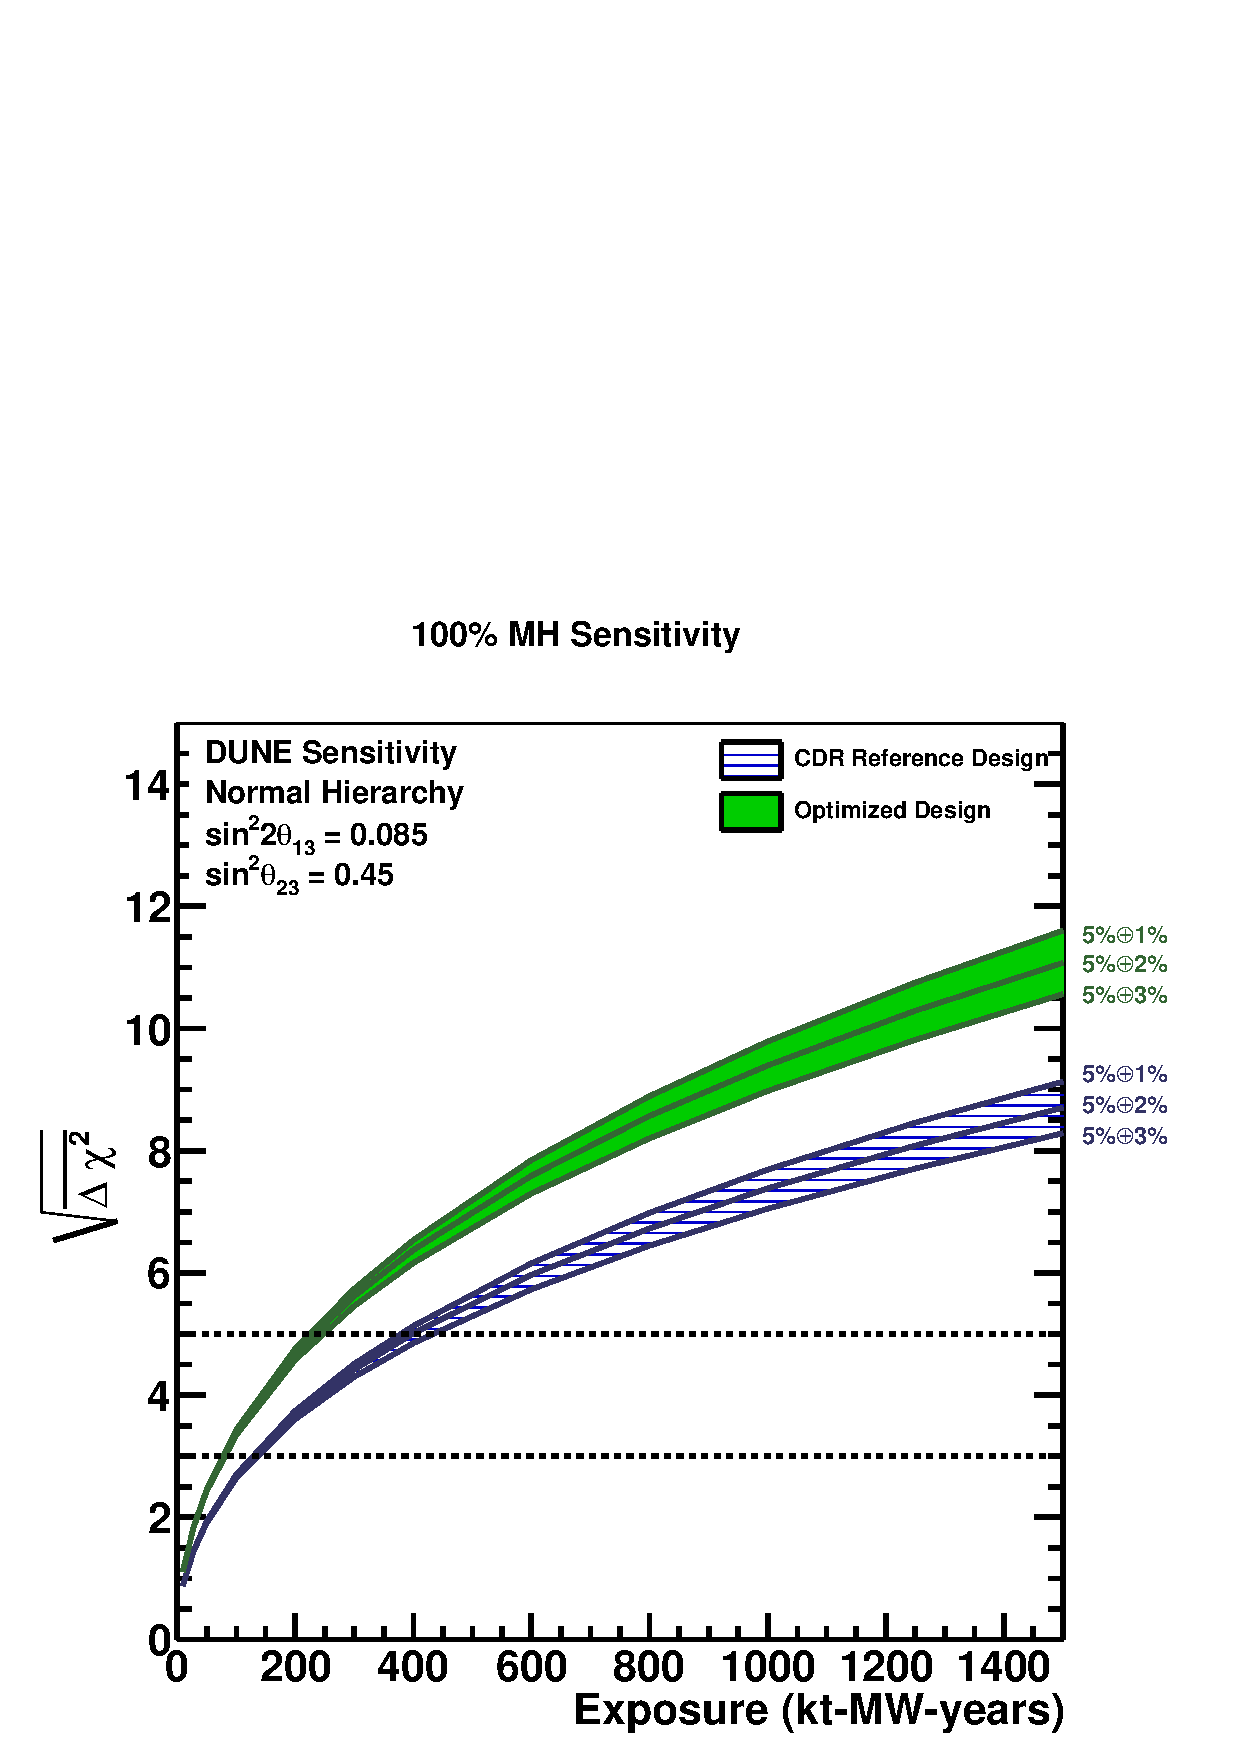
\includegraphics[width=0.45\linewidth]{volume-physics/figures/mh_exp_syst.pdf} \\
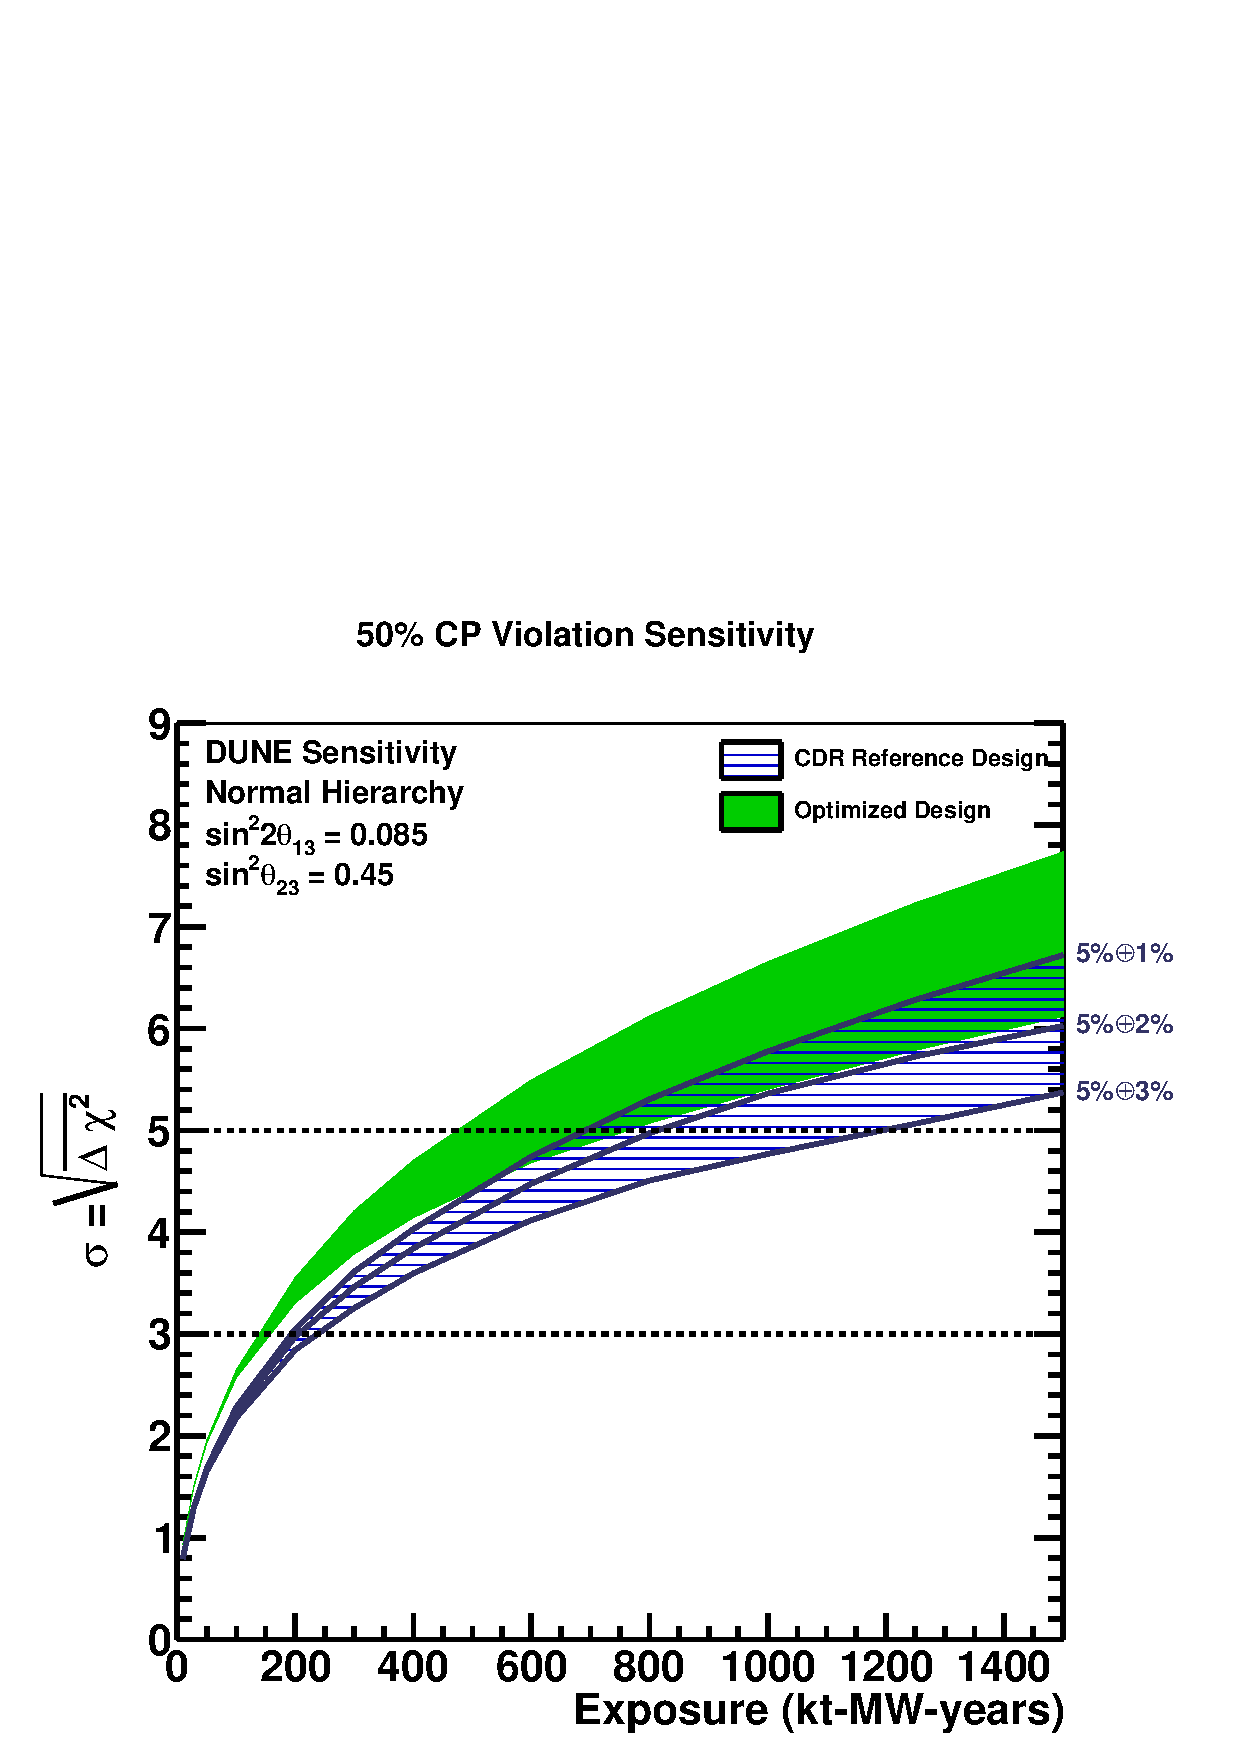
\includegraphics[width=0.45\linewidth]{volume-physics/figures/cpv50_exp_syst.pdf}
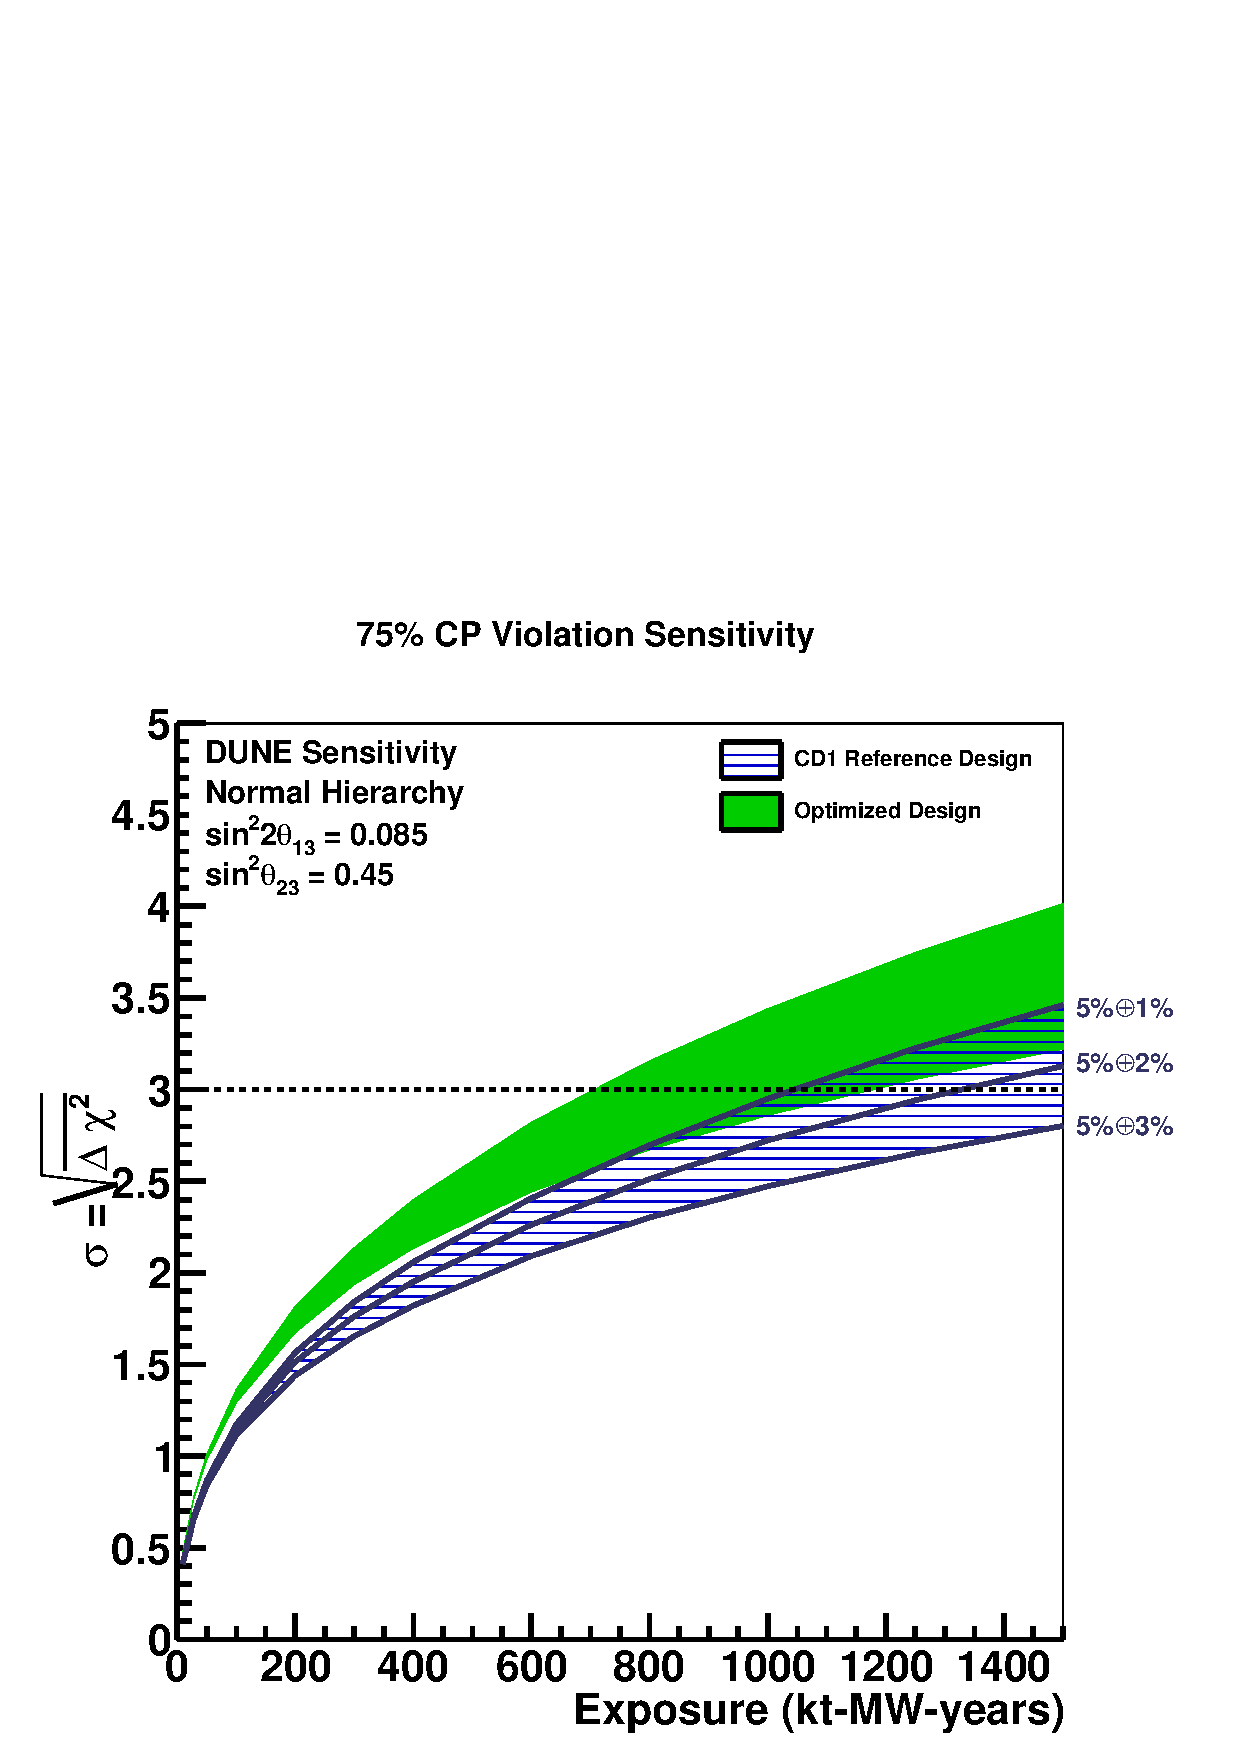
\includegraphics[width=0.45\linewidth]{volume-physics/figures/cpv75_exp_syst.pdf}
\end{cdrfigure}

Signal and
background normalization uncertainties remain
relatively unimportant for the mass hierarchy measurement, even at large exposure, when considering
minimum sensitivity for 100\% of \deltacp values. This is because the minimum sensitivity 
occurs in the near-degenerate region where it is difficult to determine
whether one is observing \deltacp $= + \pi/2 $ in the normal hierarchy
or \deltacp $=-\pi/2$ in the inverted hierarchy. Spectral analysis will
help resolve this near-degeneracy, but is dependent on as-yet
unexplored uncertainties in the spectral shape, which are expected to be dominated
by energy-scale uncertainty. Figure~\ref{fig:escale_syst} shows the
impact on MH and CP-violation sensitivity of one possible energy-scale variation, in which
energy bins are adjusted by N[E]$\rightarrow$N[(1+a)E], while keeping the total number of
events fixed. This is only one possible type of energy-scale uncertainty; more comprehensive
study of energy-scale uncertainty is in progress and will be included in
future analyses of experimental sensitivity.
%
\begin{cdrfigure}[Variation in sensitivity due to an energy-scale uncertainty]{escale_syst}{
Expected sensitivity of DUNE to determination of the neutrino mass
  hierarchy (left) and discovery of CP violation, i.e. $\delta_{CP} \ne$ 0 or $\pi$,
  (right) as a function of the true value of \deltacp, assuming 
  equal running in neutrino and antineutrino mode, for a range of values assigned to the
  ``a'' parameter in the energy-scale variation described in the text. In the MH figure, the case with no
  energy-scale systematic provides a significance of at least $\sqrt{\Delta\chi^2}$ = 5 for
  all values of \deltacp. In the CPV figure, the case with no energy-scale systematic provides
  a significance of at least 3$\sigma$ for 75\% of \deltacp values.
  (See Figures~\ref{fig:mh_exposure} and \ref{fig:cpv_exposure} for the possible range of exposures
  to achieve this level of significance.)
  Sensitivities are for true normal hierarchy; neutrino mass hierarchy
  and $\theta_{23}$ octant are assumed to be unknown.}
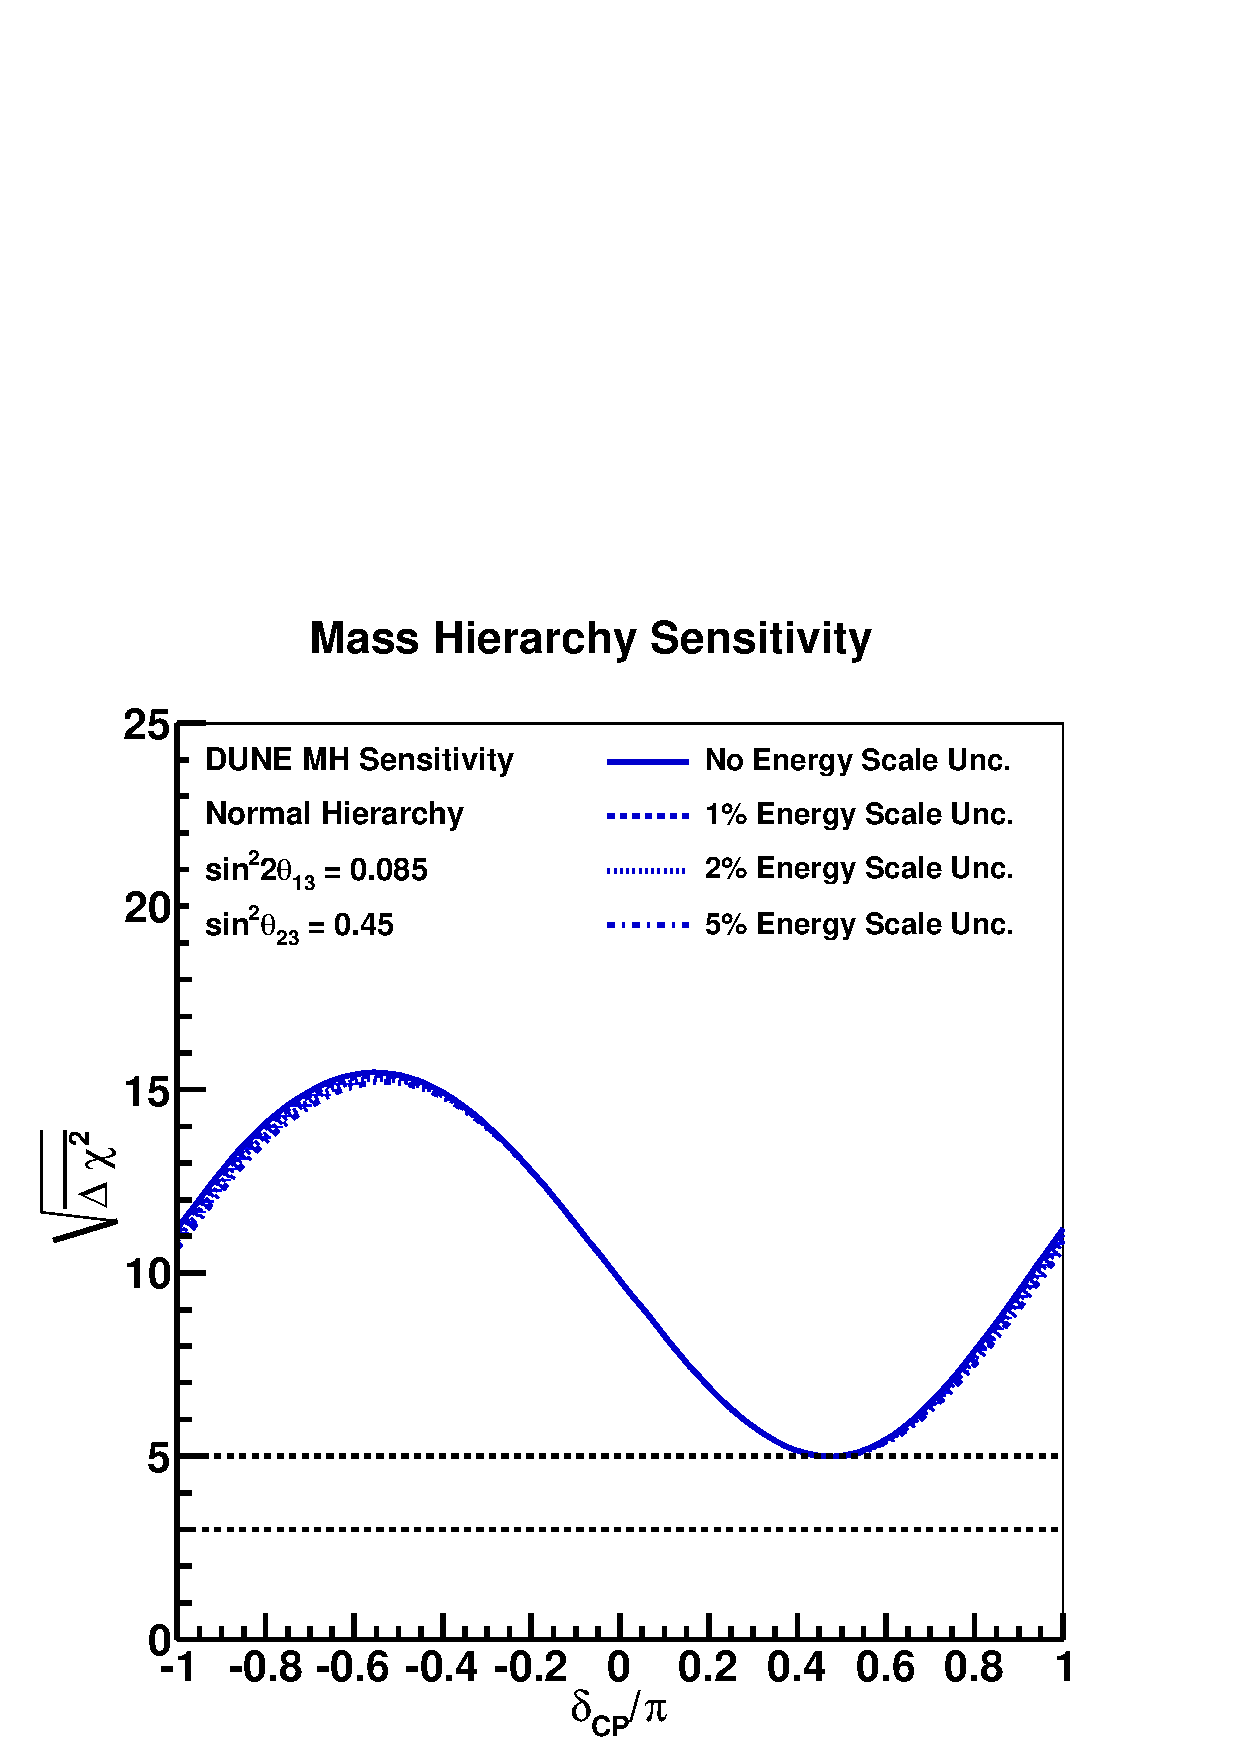
\includegraphics[width=0.44\linewidth]{volume-physics/figures/mh_230ktmwyear_varyesyst.pdf}
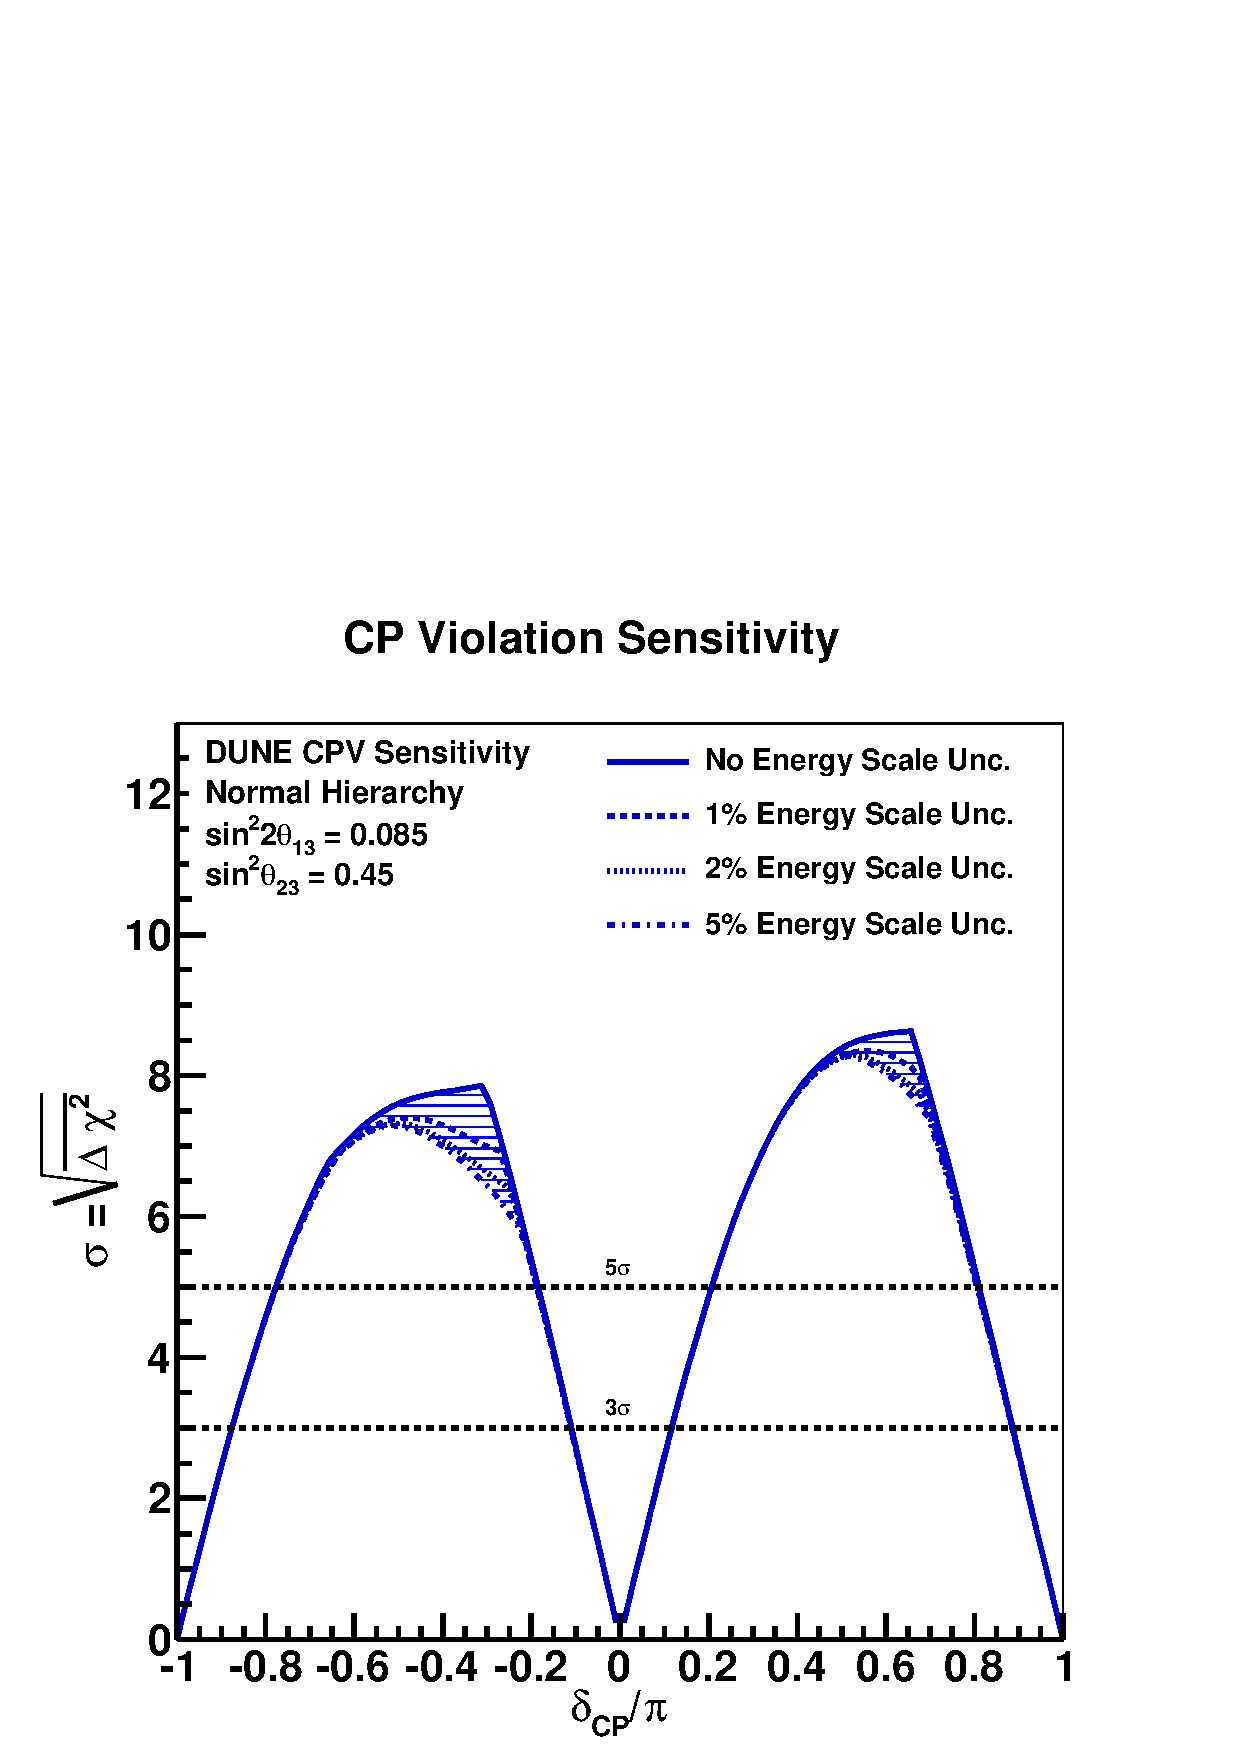
\includegraphics[width=0.44\linewidth]{volume-physics/figures/cpv_890ktmwyear_varyesyst.pdf}
\end{cdrfigure}
%
\subsection{Ongoing and Planned Studies of Systematic Uncertainty}
\label{sec:syst_studies_ind}
Detailed evaluation of systematic uncertainties for DUNE is ongoing. In many cases plans for studies
have been developed but have not yet been executed. In general, each systematic will be studied both by
propagating its uncertainty to oscillation analyses to evaluate the resultant degradation of the sensitivity
and by ensuring the considered variations give proper coverage, i.e., truly encapsulating
the lack of knowledge of the processes/effects in question. Estimates of systematic uncertainty for the 
propagation studies will be varied between the constraints available from current external knowledge
and a range of projections for ND performance. In cases where systematic uncertainty is shown to
degrade the oscillation parameter
measurement sensitivities, the required constraints will become detector performance requirements.
The details of these studies are beyond the scope of this document; however, conclusions from some
initial studies and an overview of each source of systematic uncertainty is laid out in the remainder of
this section.

Initial studies using a Near Detector Fast Monte Carlo with a parameterized detector response
predict 3\% statistical uncertainties on the absolute flux using fully 
leptonic neutrino interactions for which high-precision cross section predictions 
exist. Specifically,
the statistical uncertainty is expected to be $\sim$3\% for neutrino-electron
scattering ($E_\nu<5$~GeV) and inverse muon decay ($E_\nu>11$~GeV).
Relative normalization using the low-$\nu_0$ method is
expected to constrain the flux shape to 1--2\%; this level of
precision in the \numu flux was achieved by NOMAD\cite{Wu:2007ab,Lyubushkin:2008pe}, enabled by its 0.2\%
uncertainty in the muon energy scale. This flux shape measurement will be made for both \nue and \numu, therefore,
in combination with measurements from hadron production experiments, it can determine the distribution of
the parent mesons which will constrain the near/far flux ratio. Detailed discussion of the planned program
of ND measurements is in Chapter~\ref{ch:physics-nd} and~\cite{Mishra:2008nx,Adams:2013qkq}.
Studies using a multi-sample fit  to constrain the flux with simulated DUNE near detector
event samples show significant constraints on all flux
uncertainties; the post-fit uncertainty in most flux bins for this preliminary fit is less
than 5\%, which is the uncorrelated \numu signal normalization
uncertainty assumed by the sensitivity calculations.

%%NOTE TO EDITORS: Important to make sure that the numbers quoted in this section match those in
%%chapter-near.tex - should currently match, but if any changes are made to that section, they should
%%be propagated here.

The two main sources of uncertainty in the beam simulation come from variations in the beam optics,
$\mathcal{O}($1\%), and uncertainties in the hadron production models, $\mathcal{O}$(10\%).
Beam optics variations have been studied in detail
%, and while the variations in the flux produced by these uncertainties
%lead to large uncertainties in the FD-only fits,
and are found to be easily constrained by the ND. Software tools that
allow re-weighting of neutrinos based on their parent hadrons have been developed by \minerva; work is progressing with
them to implement these tools in the DUNE simulation to evaluate the impact of uncertainty in
hadron production models.
In the meantime, \minerva has agreed to provide its flux covariance matrix
that details the flux rate and shape uncertainties prior to ND constraints. This will be combined with DUNE
simulations to project reasonable hadron-production uncertainties to ND and FD analyses. 
Ultimately these uncertainties will be constrained by near detector measurements and
dedicated hadron-production measurements such as those at NA61/SHINE~\cite{NA61:2014fnalbeams}
will provide additional external constraints.

Primary interaction uncertainties are specific to each model, and each of the three major
cross section components (quasi-elastic processes, resonance production, and deep inelastic scattering)
contribute roughly equally to the \nue and \anue
appearance signal. In most cases, uncertainty in modeling primary interactions comes from the
hadronic interaction part of the calculation, which includes form factors in the hadron tensor,
the nuclear initial state, and FSI. 
%The later two sources of uncertainty will be discussed in the context of nuclear models later in this
%section. 

  \emph{Coherent scattering}: Coherent models built upon partially conserved axial current
  theory relate the neutrino scattering 
  cross section to pion-nucleon or pion-nucleus scattering data~\cite{Rein-Sehgal:1983}\cite{Berger-Sehgal:2009}. The choice and characterization
  of that data can have large effects on the calculated cross section. Alternate ``microscopic model'' 
  formulations are valid only over limited kinematic ranges and are not adequate to describe this process 
  for DUNE~\cite{Alvarez-Ruso-Geng-Hirenzaki-Vicente-Vacas:2007}\cite{Alvarez-Ruso-Geng-Vicente-Vacas:2007}. 
  Both types of model suffer from limited data constraints over a range of neutrino energy
  and nuclear targets. 
  However, the low hadron thresholds and good angular resolution of the DUNE ND should be able
  to produce world-leading measurements and provide adequate constraints for this interaction channel and 
  its relatively small contribution to the overall cross section. Data from \minerva~\cite{Higuera:2014azj},
  T2K, and
  upcoming LArTPC experiments will provide constraints for a variety of target nuclei over the
  relevant energy ranges required to constrain this sub-dominant process.

  \emph{Quasi-elastic processes (QE)}: Models for this type of interaction require that the target nucleon 
  is neither excited nor fragmented because the 4-momentum transfer to the hadronic system ($Q^{2}$) is low.
  For these low-$Q^{2}$ interactions, details of the nuclear initial state are important. However,
  current implementations of nuclear initial state models are inadequate, therefore the uncertainty in the only
  free parameter in the free-nucleon cross section model, $M_{A}^{QE}$, has been expanded to absorb the
  differences between simulations and $\nu$-nucleus scattering data. Better models of the nuclear
  initial state have been developed
  and are currently being implemented in GENIE and other generators. These new models will be compared with current 
  and future data from \minerva, T2K and upcoming LArTPC experiments, and the effect of variations in $M_{A}^{QE}$
  on FD spectra will be compared to the effect of introducing the new models.
  Eventually the set of models that best agrees with data will be adopted in the DUNE simulations and
  the uncertainties assigned to these models will reflect the level of agreement with data.

  \emph{Resonance production}:
  There are two important sources of uncertainty in this model. The first is the uncertainty on the free-nucleon
  cross section due to unconstrained form factors and their use as effective parameters to absorb nuclear
  modeling effects.
  The second is the disagreement in outgoing pion kinematics between simulations and data.
  Data from T2K, \minerva~\cite{Eberly:2014mra}\cite{Aliaga:2015wva}, upcoming LArTPC experiments, and the DUNE ND should provide good constraints for DUNE
  oscillation analyses, but model improvements will be required to help propagate these constraints
  to the FD signal and background predictions. Model improvements are needed for the principal interaction
  model, so-called ``background'' interactions where the pion is produced at the interaction vertex
  rather than through an intermediate $\Delta$ (or higher resonance), the interference between the two
  models, and the contributions to single-pion production from low-multiplicity DIS. Improved nuclear models
  are also required in order to estimate the impact of processes like pion-less delta decay and FSI. New models, which are
  available for some relevant regions of phase space, must be incorporated into generators and compared
  with data~\cite{Hernandez-Nieves-Valverde:2007}.

  \emph{Deep inelastic scattering (DIS)}: The inclusive DIS cross section on iron has been very well constrained by 
  data but individual final states have not. The primary source of uncertainty is in modeling the
  content and kinematics of the hadronic system as a function of its invariant mass. The resulting
  uncertainty on the DIS contribution to signal samples is relatively small, but it is nonetheless important
  to better constrain these models because the DIS contribution to background via pion production is significant.
  Data from \minerva and upcoming LArTPC experiments should help to constrain
  the exclusive cross sections, as well as nuclear effects on the inclusive cross section~\cite{Tice:2014pgu}.
  Current studies are focused on building parameterized re-weighting 
  functions for the hadronization model based on GENIE samples generated with 1$\sigma$ changes to each relevant 
  model parameter.

Nuclear models enter into the simulation of neutrino interactions both through modeling of initial-state interactions,
i.e., interactions between the neutrino and the initial state of the nucleons and virtual particles within the nucleus,
and modeling of final-state interactions (FSI), i.e., interactions of the particles exiting the
primary interaction vertex with the nuclear medium. 

  \emph{Nuclear initial state}: Uncertainties in initial-state interactions due to
  naive modeling of the environment of the nucleus have thus far been taken into account through inflation
  of the uncertainties on the free nucleon or quark interaction
  model. New models~\cite{Alvarez-Ruso-Hayato-Nieves:2014} are being added to generators and will soon be incorporated into the Fast MC
  to study how the impact on sensitivity of these models compares with uncertainties in the current nominal model.
  Data from upcoming LArTPC neutrino experiments will provide detailed information on nucleon production
  rates and kinematics, which will help to distinguish which of the new models best describes the data.

  \emph{Final-state interactions}: FSI can alter event reconstruction in two distinct ways. The first is a smearing
  of the total energy available to be deposited in the detector. The second is the misidentification of
  event topologies used to classify the neutrino flavor and interaction mode. Uncertainties in selection
  efficiencies and event-sample migrations
  due to intranuclear rescattering can be studied with existing DUNE tools. The predictions and
  uncertainties on GENIE's ``hA'' model~\cite{Dytman:2011zz} of intranuclear interaction
  are being tested against the detailed FSI model in the GiBUU~\cite{Buss:2011mx} event
  generator. Studies of correlations among the free model parameters and and how variations in those
  parameters propagate differently for $\nu$ and $\bar{\nu}$ are also needed. 
  Electron-argon scattering data~\cite{Benhar:2014nca}  and studies of hadron production
  in upcoming LArTPC experiments are expected to further constrain the effects of FSI in argon nuclei.

A fit to Fast MC simulation of all four far detector samples
(\nue, \anue, \numu, \anumu) significantly
constrains cross section systematic uncertainty even in the case where many
cross section parameters are allowed to vary simultaneously within their
GENIE uncertainties. As seen in the example shown in Figure
\ref{fig:MAresqesyst}, 
a fit in which both $M_A^{QE,CC}$ and 
$M_A^{RES,CC}$ are allowed to vary within their GENIE uncertainties 
($\pm$20\%), which could significantly alter the energy distribution of the 
the selected events, results in a dramatic reduction in sensitivity if one 
considers only the $\nu_e$ appearance signal without constraint from the 
$\bar{\nu}_e$ and $\nu_{\mu}$/$\bar{\nu}_{\mu}$ samples.
In contrast, for a four sample fit,
this same parameter variation results in a smaller reduction in
sensitivity to CP violation.
This result includes a 10\% uncertainty in the $\nu/\bar{\nu}$
cross section ratio and a 2.5\% uncertainty in the $\nu_e/\nu_{\mu}$
cross section ratio; uncertainties in these ratios as large as 20\% have
been considered and did not produce dramatically different results.
More details on this analysis are available in \cite{Bass:2014vta}.
Preliminary studies also demonstrate significant constraint on cross section systematics
from the near detector.
%
\begin{cdrfigure}[Example of cross section uncertainty cancellation in FD fit]{MAresqesyst}{
An example CP violation sensitivity calculated using inputs from the 
  FastMC in a fit to all four ($\nu_e$, $\overline\nu_e$, $\nu_{\mu}$, 
  $\overline\nu_{\mu}$) samples (red) and a fit to the $\nu_e$ appearance sample 
  only (blue), for the case of no systematic uncertainty (solid) and the case in
  which both $M_A^{QE,CC}$ and $M_A^{RES,CC}$ are allowed to vary with a
  1$\sigma$ uncertainty of 20\% (dashed). This example was taken from an earlier
  DUNE study, so the absolute sensitivity can not be compared with the DUNE 
  sensitivities presented in this document.}
\includegraphics[width=0.5\linewidth]{volume-physics/figures/cpv_QELCCMA_RESCCMA.pdf}
\end{cdrfigure}

Uncertainty stemming from detector effects
are somewhat more difficult to address with existing
simulation efforts. Tools to evaluate the effect of uncertainty in single-particle resolutions,
detection and particle-identification efficiencies, and energy scale are in development within
the Fast MC framework. The results of these studies will provide performance requirements
for the DUNE detectors, but more complete understanding of the expected size of these effects
will require comparison between data and a full Monte Carlo.
The status of efforts to develop reconstruction and analysis tools for a full Monte Carlo simulation
of DUNE is described in %Section~\ref{sec:detectors-sc-physics-software}
the Software and Computing chapter of \voldune. At the same time,
a number of test-beam and prototype experiments, including the DUNE 35-t prototype,
LARIAT, CAPTAIN, and the CERN neutrino platform experiments, are being designed and built to reduce these
uncertainties with experimental data. The status of some of these efforts is described in the Prototyping
Strategy chapter of \voldune.
%Chapter~\ref{ch:detectors-proto}.

These ongoing studies to improve models of neutrino interactions in LArTPC detectors and
to evaluate the remaining uncertainties, by comparisons to data and alternate models, 
%are a high priority of the whole neutrino community as well as the DUNE collaboration.
are considered high priority not only by the DUNE collaboration, but by the global neutrino community.
It is reasonable to expect that model improvements and new data will provide DUNE with improved inputs
and reduced uncertainties compared to current knowledge. Following the plan described in the preceding
paragraphs, DUNE collaborators will actively participate in the global effort to improve understanding
of neutrino interactions, will propagate what is learned
in the intermediate neutrino program to DUNE analyses, and will
evaluate the effect of remaining uncertainties on the DUNE analyses.











